\chapter{Algorithmen zur Erkennung von SLTRs}\label{main_algo}

Im vorherigen Kapitel wurden Kriterien für die Existenz einer SLTR für $G$ erarbeitet. Angenommen, wir haben nun einen intern-3-zusammenhängenden ebenen Graphen $G$ mit Aufhängungen $a_1,a_2$ und $a_3$ gegeben und wollen die Frage beantworten, ob dieser spezifische Graph eine SLTR hat.

Die beiden Hauptresultate aus Kapitel \ref{main_theory} geben uns jeweils die Möglichkeit für ein spezifisches FAA zu überprüfen, ob es eine SLTR induziert. Da es aber Graphen mit exponentiell vielen FAAs gibt, wie in Beispiel \ref{bsp_faa} gezeigt wurde, ist dies kein effizienter Weg, um die Frage zu beantworten. Im Falle der Ecken-Kompatibilität lässt sich dieses Vorgehen auch umkehren. Wir können für jeden Schnyder Wood überprüfen, ob zu diesem ein Ecken kompatibles FAA auf $G$ existiert. Zumindest für Graphen, die nur polynominell viele Schnyder Woods haben, erhalten wir nach Aerts und Felsner so einen polynominellen Algorithmus, indem wir ein Matching-Problem lösen \cite{af15}. Es existieren allerdings Graphen auf $n$ Knoten mit $3.209^n$ vielen Schnyder Woods wie Felsner und Zinkfeld gezeigt haben \cite{fz08}. Es ist also nicht möglich, mit diesen Ansätzen einen Algorithmus zu konstruieren, um die Frage nach der Existenz einer SLTR effizient zu beantworten.

Um dies jedoch zu erreichen, werden wir uns in diesem Kapitel mit einem von Aerts und Felsner erarbeiteten Algorithmus beschäftigen \cite{af15}. Dieser Algorithmus charakterisiert die Antwort der oben gestellten Frage als ganzzahlige Lösung eines Gerichteten-Multi-Fluss-Problems. Wir stellen am Ende des Kapitels die Vermutung auf, dass man mithilfe dieses Ansatzes einen polynominellen deterministischen Algorithmus zur Bestimmung von SLTRs konstruieren kann.

\section{SLTRs als Lösungen eines Zwei-Fluss-Problems}

In einem ersten Schritt werden wir für einen gegebenen intern-3-zusammenhängenden ebenen Graphen $G$ mit Aufhängungen $a_1,a_2,a_3$, sowohl einen Schnyder Wood als auch ein FAA jeweils als ganzzahlige Lösung eines Gerichteten-Ein-Fluss-Problems charakterisieren. Die beiden so konstruierten Netzwerke werden dann zu einem Gerichteten-Zwei-Fluss-Problem kombiniert, sodass eine zulässige ganzzahlige Lösung einem Ecken kompatiblen Paar auf $G$ entspricht. Als Resultat erhalten wir eine SLTR von $G$. Wir beschäftigen uns also im Verlauf den Kapitels mit verschiedenen Multi-Fluss-Problemen auf gerichteten Graphen, die wir in Definition \ref{def_multi_flow} eingeführt haben.

\subsection{Schnyder-Wood-Fluss}

Um einen Schnyder Wood als Fluss-Problem zu kodieren, kann man die in Abschnitt \ref{alpha_orientations} eingeführten $\alpha_s$-Orientierungen auf dem Abschluss von $G+G^*$ nutzen. \'Eric Fusy zeigt im Zuge der Untersuchung spezifischer $\alpha$-Funktionen, dass sich $\alpha_s$-Orientierungen von $G+G^*$ in linearer Zeit berechnen lassen\cite{fusy07}. Daraus folgt, dass wir auch einen Schnyder Wood auf $G$ in linearer Zeit erhalten. 

Sei ein ebener intern-3-zusammenhängender Graph $G$ mit Aufhängungen $a_1,a_2,a_3$ gegeben. Machen wir uns an die Konstruktion eines Netzwerks $\mathcal{N}_S$, sodass ein zulässiger ganzzahliger Fluss $\varphi_s$ auf $\mathcal{N}_S$ einer $\alpha_s$-Orientierung von $G+G^*$ entspricht\footnote{Hier stehen die drei \textit{s} jeweils für Schnyder Wood um spätere Verwechslungen zu vermeiden.}. Nach Theorem \ref{alpha_bij} würde die aus $\varphi_s$ erhaltene $\alpha_s$-Orientierung somit auch einen Schnyder Wood auf $G$ induzieren. Besonderes Augenmerk ist hier auf die Möglichkeit einer späteren Kombination mit einem weiteren Netzwerk gelegt, in welchem eine ganzzahlige Lösung einem FAA auf $G$ entspricht, um ein kombiniertes Netzwerk zu erstellen.

Wie schon erwähnt ist $G+G^*$ bipartit, Kanten-Knoten haben Grad 4, Knoten-Knoten haben Grad $\text{deg}(v)$ und Gebiets-Knoten haben Grad $|f|$. Für eine $\alpha_s$-Orien\-tier\-ung muss nach Theorem \ref{alpha_bij} A3 jeder Kanten-Knoten Ausgangsgrad 1, jeder Knoten-Knoten Eingangsgrad $\text{deg}(v)-3$ und jeder Gebiets-Knoten Eingangsgrad $|f|-3$ haben. Die Kanten-Knoten am äußeren Gebiet sind in $G+G^*$ immer nach außen orientiert. Somit reicht es, wenn wir nur die inneren Kanten-Kanten $E_{in}$ betrachten und die Orientierung der äußeren Kanten voraussetzten.

\begin{figure}
	\centering
  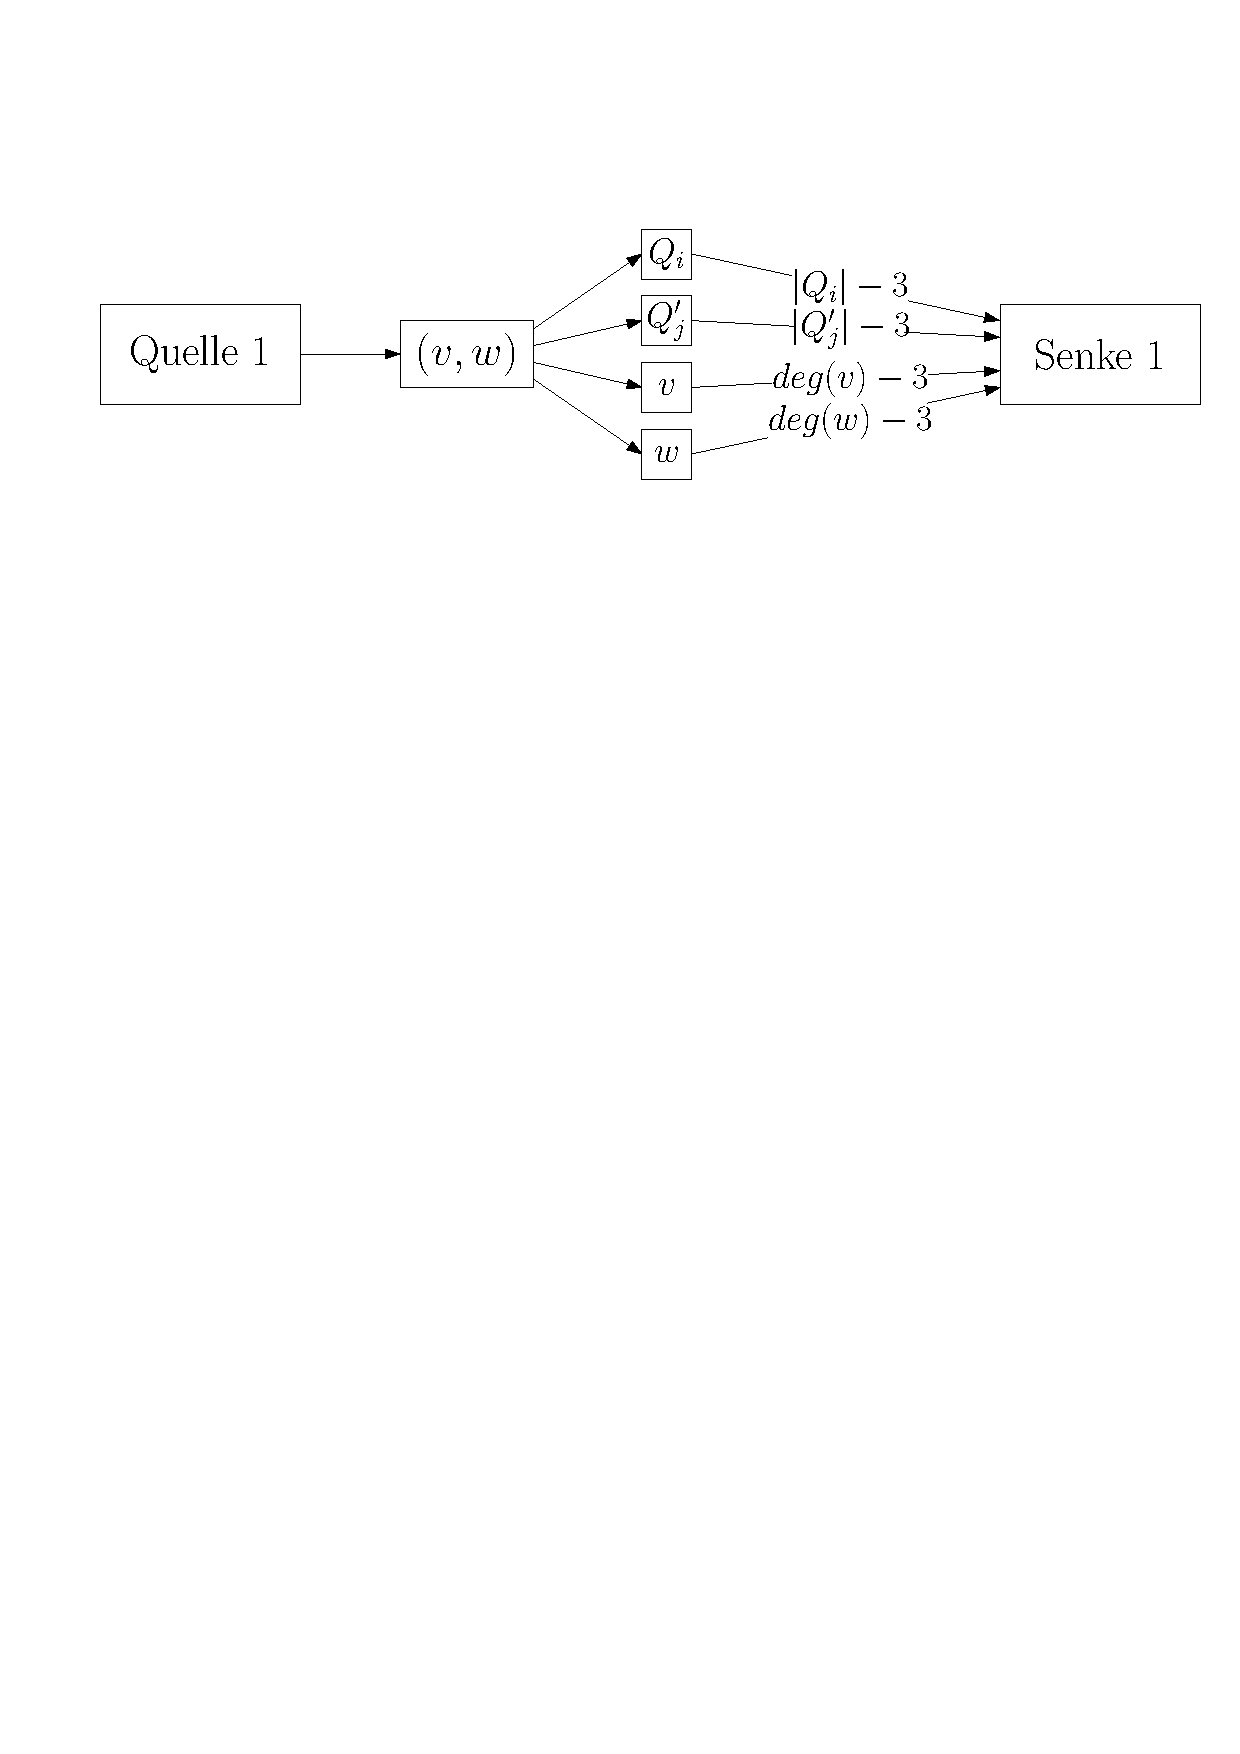
\includegraphics[width=0.9\textwidth]{schnyder_flow.pdf}
  \caption{Der Schnyder Wood Fluss durch eine innere Kante $(v,w)$. Die nicht beschrifteten Kanten haben Kapazität 1.}
  \label{schnyder_flow}
\end{figure}

Das im Folgenden konstruierte Netzwerk ist in Abbildung \ref{schnyder_flow} skizziert und unter dem Punkt Netzwerk \ref{net_schnyder} zusammengefasst. Das Netzwerk $\mathcal{N}_S$ hat eine Quelle $s$ und eine Senke $t$ und einen Knoten für jeden Knoten aus $G+G^*$ (bis auf die äußeren Kanten). Es existieren Kanten von der Quelle zu jedem Kanten-Knoten $e \in E_{in}$ mit Kapazität 1. Von den Kanten-Knoten $e$ zu inzidenten Knoten-Knoten $v$ und Gebiets-Knoten $f \in F_{in}$ fügen wir ebenfalls Kanten mit Kapazität 1 ein. Merke, dass der Fluss auf diesen Kanten bei einer ganzzahligen Lösung eine $\alpha_s$-Orientierung auf $G+G^*$ ergeben soll. Nun fügen wir noch Kanten von $f \in F_{in}$ zur Senke mit Kapazitäten $|f|-3$, Kanten von den (inneren) Knoten-Knoten $v \in V_{in} = V \setminus \{a_1,a_2,a_3\}$ zur Senke mit Kapazitäten $\text{deg}(v)-3$ und Kanten von den Aufhängungen $a_i$ zur Senke mit Kapazitäten $\text{deg}(a_i)-2$. Die letzte Kapazität ergibt sich, da die Halbkante in $G+G^*$ von $a_i$ aus immer nach außen orientiert. Wir müssen somit nur noch zwei andere Kanten von $a_i$ weg orientieren. Der Bedarf des Netzwerkes entspricht der Anzahl der inneren Kanten von $G$. Fassen wir zusammen.

\begin{network}[Schnyder Wood]\label{net_schnyder}
Bei $\mathcal{N}_S$ handelt es sich um ein gerichtetes Netzwerk, das auf Basis eines ebenen intern-3-zusammenhängenden Graphen $G$ mit Aufhängungen $a_1,a_2,a_3$ erstellt wird, um einen Schnyder Wood auf $G$ zu finden. Ein Ausschnitt ist in Abbildung \ref{schnyder_flow} dargestellt.
	\begin{itemize}
	\item $\mathcal{N}_S$ hat eine Quelle $s$ und eine Senke $t$
	\item Knoten in $\mathcal{N}_S$ werden für jede innere Kante $e \in E_{in}$, jedes innere Gebiet $f\in F_{in}$ und jeden Knoten $v \in V$ aus $G$ erzeugt.
	\item Es werden gerichtete Kanten der folgenden Typen in $\mathcal{N}_S$ erzeugt:
		\begin{itemize}
		\item $(s,e)$ von der Quelle zu jeder inneren Kante mit $c\big(s,e\big) = 1$
		\item $(e,v_1),(e,v_2)$ von jeder inneren Kante zu den Endknoten mit $c\big(e,v\big) = 1$
		\item $(e,f)$ von jeder inneren Kante zu adjazenten Gebieten mit $c\big(e,f\big) = 1$
		\item $(v,t)$ von den Knoten zur Senke mit $c\big(v,t\big) = 1$
		\item $(f,t)$ von den inneren Gebieten zur Senke mit $c\big(f,t\big) = |f|-3$
		\item $(a_i,t)$ von den Aufhängungen zur Senke mit $c\big(f,t\big) = \text{deg}(a_i)-2$
		\item $(v,t)$ von den restlichen Knoten zur Senke mit $c\big(f,t\big) = \text{deg}(v)-3$
		\end{itemize}
	\item $\mathcal{N}_S$ hat Bedarf $d=|E_{in}|$
	\item [$\Rightarrow$] Ein zulässiger ganzzahliger Fluss $\varphi_s$ existiert genau dann, wenn ein Schnyder Wood  auf $G$ existiert.
	\end{itemize}
\end{network}

\begin{proposition}
Sei $G$ ein ebener intern-3-zusammenhängender Graph mit Aufhängungen $a_1,a_2,a_3$ und $\mathcal{N}_S$ wie in Netzwerk \ref{net_schnyder} konstruiert. Ein zulässiger ganzzahliger Fluss $\varphi_s$ auf $\mathcal{N}_S$ existiert genau dann, wenn ein Schnyder Wood auf $G$ zu den Aufhängungen $a_1,a_2,a_3$ existiert. Insbesondere kodiert jeder Fluss einen Schnyder Wood.
\end{proposition}

\begin{proof}
Sei $\varphi_s$ ein zulässiger ganzzahliger Fluss auf $\mathcal{N}_S$. Es gilt $|\varphi_s| = |E_{in}|$. Somit hat jede innere Kante-Knoten Ausgangsgrad 1. Weiter gilt 
$$\sum_{v \in V} \Big(\text{deg}(v)-3\Big) + 3 + \sum_{f \in F_{in}} \Big(|f|-3\Big) = |E_{in}|.$$
Somit sind die Kanten von den Kanten-Knoten und Knoten-Knoten ausgelastet. Der Fluss $\varphi_s$ entlang einer Auskante von $e \in E_{in}$ in $\mathcal{N}_S$ entspricht dann genau der Kante in $G+G^*$, die in der $\alpha_{s}$-Orientierung von $e$ weg orientiert wird. Durch die Knoten-Knoten $v$ und Gebiets-Knoten $f$ fließt Fluss auf $\text{deg}(v)-3$ bzw. $|f|-3$ Kanten der von den Kanten-Knoten kommt. Somit lässt $\varphi_s$ jeweils drei Kanten frei, denen wir noch keine Orientierung zugewiesen haben. Diese entsprechen somit den von $v$ bzw. $f$ weg orientierten Kanten einer $\alpha_{s}$-Orientierung auf $G+G^*$. Somit hat jedes Gebiet und jeder Knoten den passenden Ausgangsgrad und $\varphi_s$ kodiert eine $\alpha_s$-Orientierung auf $G+G^*$. Auf analoge Weise lässt sich aus einer $\alpha_s$-Orientierung ein zulässiger ganzzahliger Fluss $\varphi_s$ erstellen. Es existiert also genau dann ein Schnyder Wood auf $G$, wenn eine ganzzahlige Lösung $\varphi_s$ für $\mathcal{N}_S$ existiert.
\end{proof}

\subsection{FAA-Fluss}\label{faa-flow}

Sei wieder ein ebener intern-3-zusammenhängender Graph $G$ mit Aufhängungen $a_1,a_2,a_3$ gegeben. Ein FAA ordnet nun jedem Gebiet $|f|-3$ flache Winkel zu und jeder Knoten darf maximal einem Gebiet zugeordnet werden. Die adjazenten Knoten um das äußere Gebiet, die keine Aufhängungen sind, müssen diesem zugewiesen werden. Wir konstruieren ein Netzwerk $\mathcal{N}_F$, für das ein ganzzahliger zulässiger Fluss einem FAA entspricht 

\begin{figure}
	\centering
  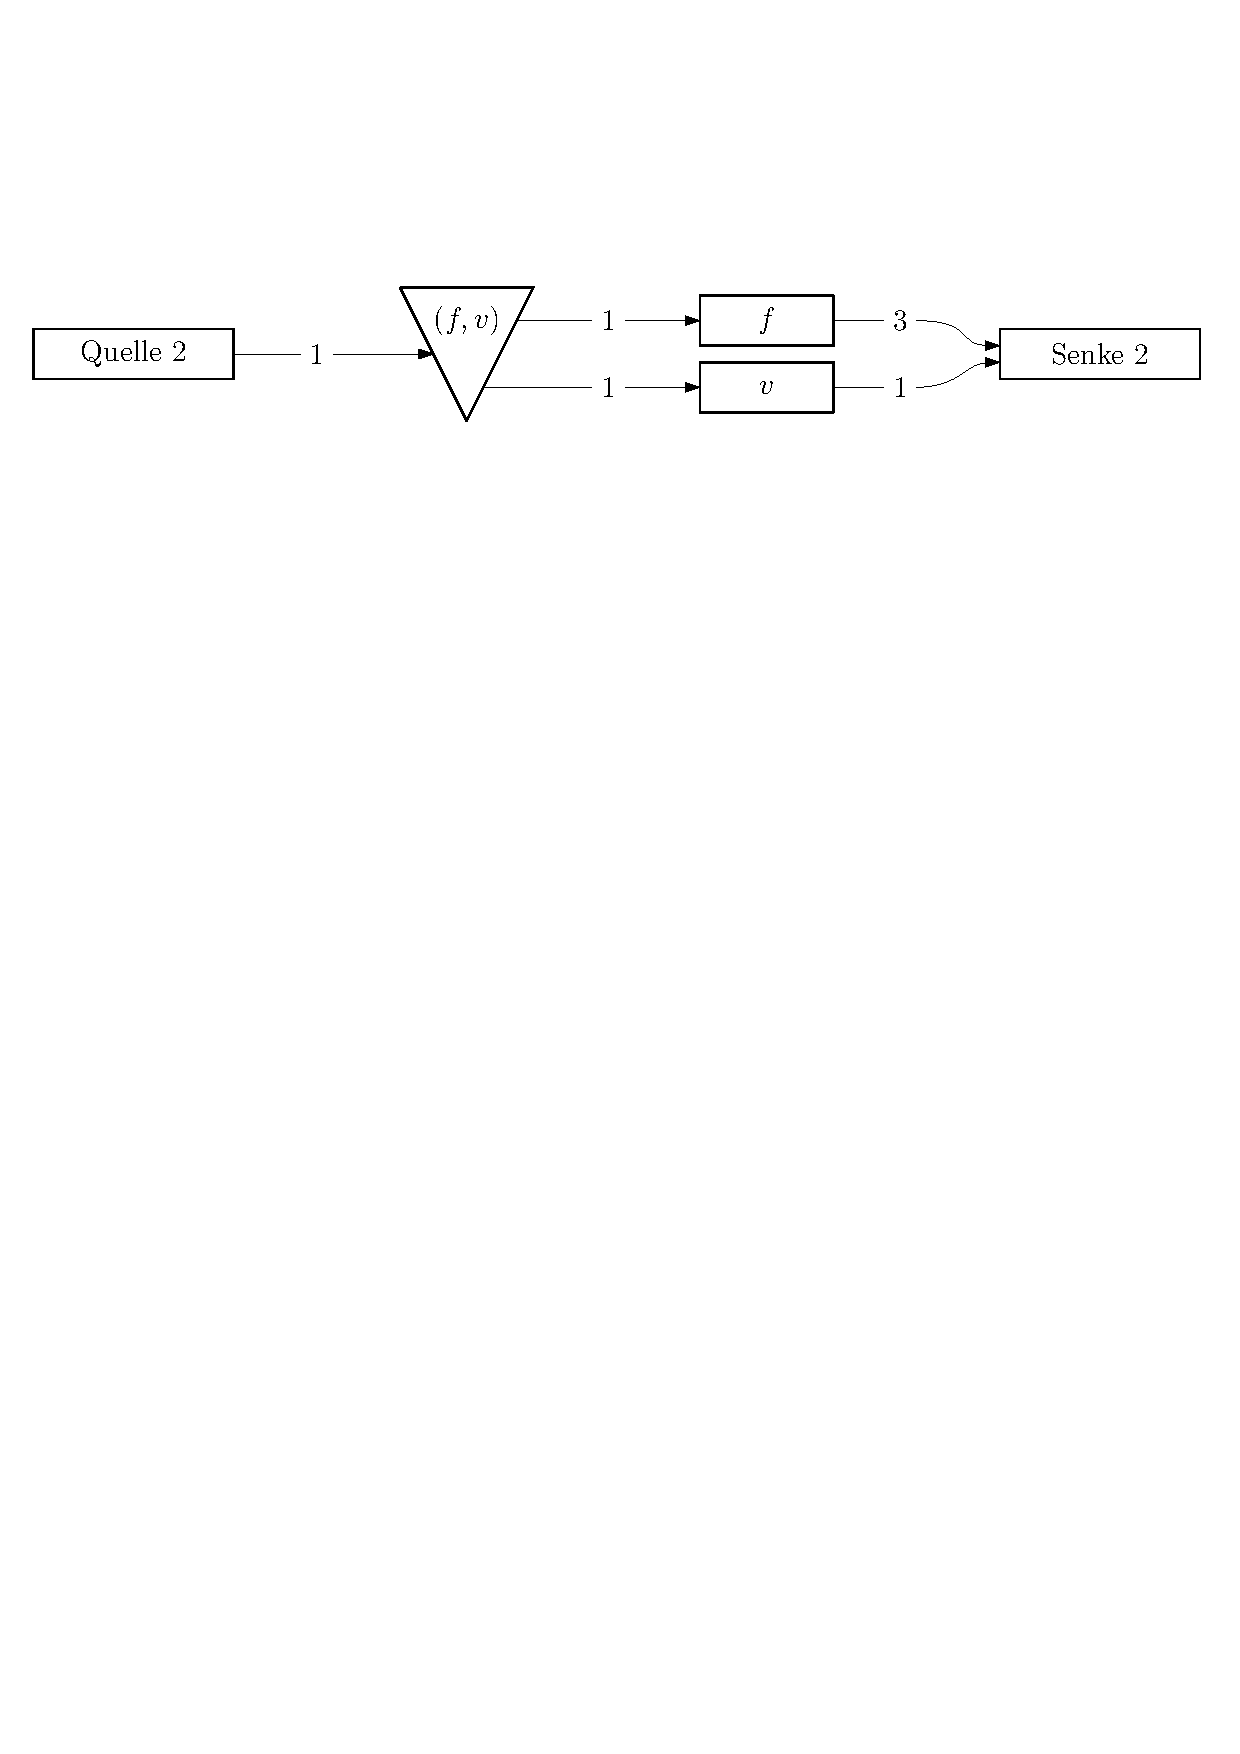
\includegraphics[width=1\textwidth]{faa_flow.pdf}
  \caption{Der FAA-Fluss durch einen Winkel $(f,v)$. Die nicht beschrifteten Kanten haben Kapazität 1.}
  \label{faa_flow}
\end{figure}

Das im Folgenden konstruierte Netzwerk ist in Abbildung \ref{faa_flow} skizziert und unter dem Punkt Netzwerk \ref{net_faa} zusammengefasst. Das Netzwerk $\mathcal{N}_F$ hat jeweils eine Quelle und Senke. Wir erstellen in $\mathcal{N}_F$ Knoten für jeden inneren Winkel $(f,v)$, mit $v\in V$ und $f \in F_{in}$, Knoten für alle inneren Gebiete $f \in F_{in}$ und für die inneren Knoten $v\in V_{in}$. Von der Quelle fügen wir Kanten mit Kapazität 1 zu jedem inneren Winkel $(f,v)$, und von jedem inneren Winkel $(f,v)$ jeweils eine Kante zu $f$ und zu $v$ (falls $v\in V_{in}$) mit Kapazität 1 ein. Merke, dass so der Fluss von den Winkeln zu den inneren Knoten einem FAA entspricht. Zuletzt erstellen wir Kanten von jedem inneren Gebiet $f$ zur Senke mit Kapazität 3 und Kanten von jedem Knoten $v$ zur Senke mit Kapazität 1 ein. Der Bedarf des Netzwerks ist $\sum_{f \in F_{in}}|f|$ und entspricht der Anzahl der inneren Winkel von $G$. Fassen wir zusammen.

\begin{network}[FAA]\label{net_faa}
Bei $\mathcal{N}_F$ handelt es sich um ein gerichtetes Netzwerk, das auf Basis eines ebenen intern-3-zusammenhängenden Graphen $G$ mit Aufhängungen $a_1,a_2,a_3$ erstellt wird, um ein FAA zu finden. Ein Ausschnitt ist in Abbildung \ref{faa_flow} dargestellt.
	\begin{itemize}
	\item $\mathcal{N}_F$ hat eine Quelle $s$ und eine Senke $t$
	\item Knoten in $\mathcal{N}_F$ werden für jeden inneren Winkel $(f,v) \in W_{in}$, jedes innere Gebiet $f\in F_{in}$ und jeden Knoten $v \in V$ aus $G$ erzeugt.
	\item Es werden gerichtete Kanten der folgenden Typen in $\mathcal{N}_F$ erzeugt:
		\begin{itemize}
		\item $(s,(f,v))$ von der Quelle zu jedem inneren Winkel mit $c\big(s,(f,v)\big) = 1$
		\item $((f,v),v)$ von jedem inneren Winkel zum Knoten mit $c\big((f,v),v\big) = 1$
		\item $((f,v),f)$ von jedem inneren Winkel zum Gebiet mit $c\big((f,v),f\big) = 1$
		\item $(f,t)$ von den inneren Gebieten zur Senke mit $c\big(f,t\big) = 3$
		\item $(v,t)$ von den Knoten zur Senke mit $c\big(f,t\big) = 1$
		\end{itemize}
	\item $\mathcal{N}_F$ hat Bedarf $d=\sum_{f \in F_{in}}|f|$
	\item [$\Rightarrow$]Ein zulässiger ganzzahliger Fluss $\varphi_F$ existiert genau dann, wenn ein FAA existiert.
	\end{itemize}
\end{network}

\begin{proposition}\label{prop_net_faa}
Sei $G$ ein ebener intern-3-zusammenhängender Graph mit Aufhängungen $a_1,a_2,a_3$ und $\mathcal{N}_F$ wie in Netzwerk \ref{net_faa} konstruiert. Ein zulässiger ganzzahliger Fluss $\varphi_F$ auf $\mathcal{N}_S$ existiert genau dann, wenn ein FAA auf $G$ zu den Aufhängungen $a_1,a_2,a_3$ existiert. Insbesondere kodiert jeder Fluss genau ein FAA.
\end{proposition}

\begin{proof}
Sei $\varphi_F$ ein zulässiger ganzzahliger Fluss auf $\mathcal{N}_F$. Der Fluss auf einer Kante $((f,v),f)$ entspricht einer Ecke von $f$ und Fluss auf $((f,v),u)$ der Zuweisung eines Knoten zu $f$. Zur Vereinfachung sprechen wir im Weiteren auch von Ecken- und Zuweisungs-Fluss. Somit wird jeder innere Winkel von $\varphi_F$ entweder einem Gebiet zugewiesen oder als Ecke ausgezeichnet. Da die Kanten von den inneren Knoten zur Senke Kapazität eins haben, kann jeder Knoten nur einmal zugewiesen werden. F2 ist somit erfüllt. Von jedem inneren Gebiet $f$ fließt Fluss mit Stärke $|\varphi_s(f,t)| = 3$ zur Senke. Somit muss $|f|-3$ Fluss durch zugewiesene Knoten gehen. F1 ist somit erfüllt. $\varphi_F$ respektiert also die Bedingungen aus Definition \ref{def_faa} und es existieren nur dann FAAs auf $G$, wenn mindestens eine ganzzahlige Lösung für $\mathcal{N}_F$ existiert.
\end{proof}

\begin{remark}

Das oben eingeführte Netzwerk \ref{net_faa} zur Bestimmung von FAAs lässt sich auch als Zwei-Fluss-Problem konstruieren. Wir trennen für Ecken- und Zuweisungs-Fluss die Quellen und Senken.  Zu jedem Winkelknoten $(f,v)$ fügen wir eine Kopie $(f,v)'$ ein und verbinden beide durch eine Kante mit Kapazität 1 (siehe Abbildung \ref{faa_as_2}). In den ersten Winkelknoten führt eine Kante von beiden Quellen mit Kapazität 1 und vom zweiten Knoten führen Kanten zu $f$ und $v$. Der Bedarf des Ecken-Flusses ist dann $3|F_{in}|$ und der Bedarf des Zuweisung-Flusses $\sum_{f \in F_{in}}{|f|-3}$.

\begin{figure}[b]
	\centering
  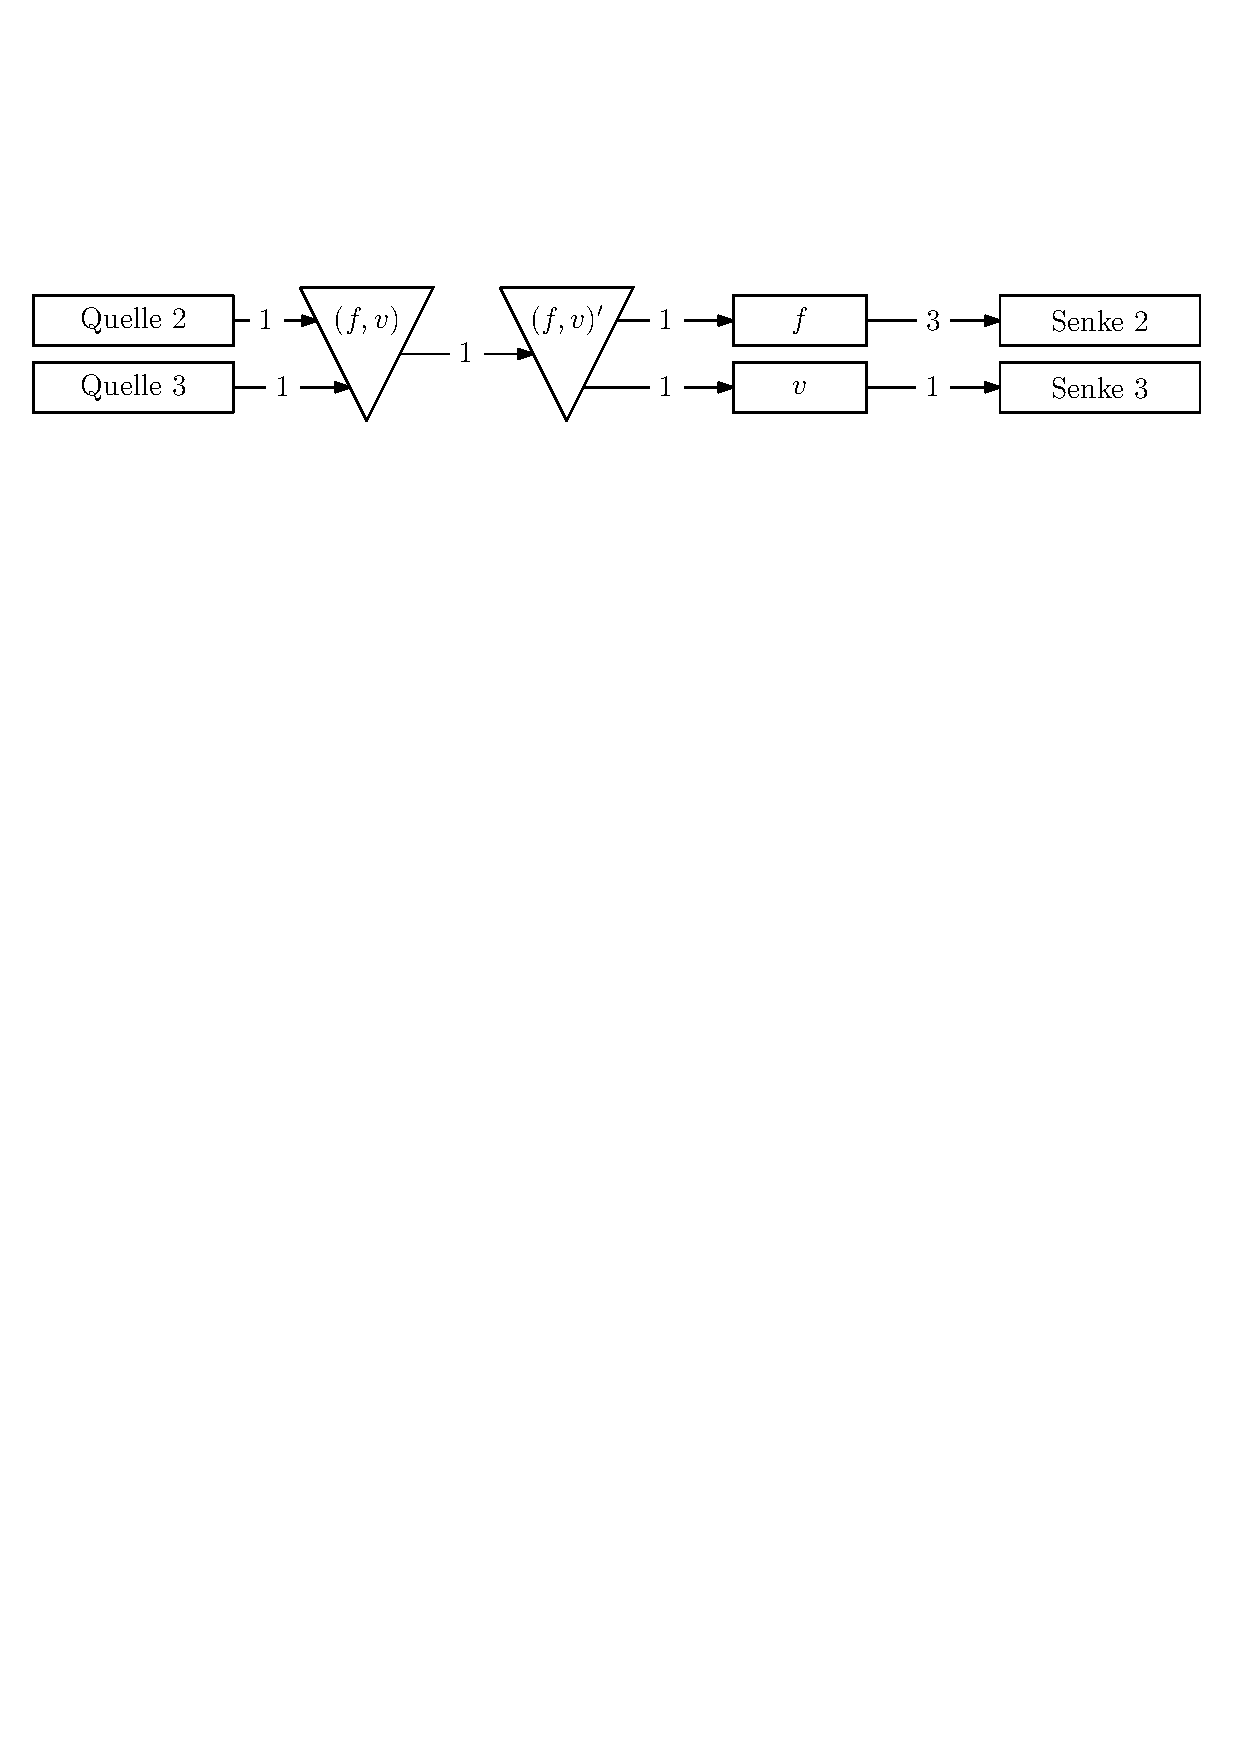
\includegraphics[width=1\textwidth]{faa_2_flow.pdf}
  \caption{Das Einfügen einer Kante und eines zweiten Winkelknotens gewährt die Trennung von Winkel- und Zuweisungs-Fluss. Die nicht beschrifteten Kanten haben Kapazität 1.}
  \label{faa_as_2}
\end{figure}

Eine zulässige ganzzahlige Lösung $\varphi_F = (\varphi_e,\varphi_z)$ entspricht dann wieder einem FAA auf $G$. Aus der Ganzzahligkeit folgt, dass ein Winkel entweder von $\varphi_{e}$ (Ecke) oder $\varphi_{z}$ (Zuweisung) genutzt wird. Dies gewährleisten die Kanten zwischen den Winkelknoten, da sie immer nur von einem der beiden Flüssen genutzt werden können.
\end{remark}

\subsection{Ein Zwei-Fluss Netzwerk zur Erkennung von SLTRs}

Im Verlauf des Kapitels haben wir nun sowohl für Schnyder Woods als auch für FAAs Netzwerke konstruiert, für die ein ganzzahliger zulässiger Fluss einem Schnyder Wood bzw. einem FAA für einen gegebenen Graphen $G$ liefert. Wir wollen jetzt eine Kombination aus beiden erstellen, die ein Ecken kompatibles Paar $(\sigma,\phi)$ aus einem Schnyder Labeling $\sigma$ und einem FAA $\phi$  kodiert. Es folgt die Konstruktion eines Netzwerkes. Wir bezeichnen es mit $\mathcal{N}_G$, welches diese Anforderung erfüllt. Ein ganzzahliger Fluss $\varphi$ kodiert dann ein Ecken kompatibles Paar und impliziert somit nach Theorem \ref{theo_ccc} eine SLTR für $G$. Dieses Netzwerk wird zwei Paare von Quellen und Senken haben. Es entspricht somit einem Gerichteten-Multi-Fluss-Problem. Wir werden nach der Konstruktion auch kurz darauf eingehen, warum sich nach diesem Ansatz kein Netzwerk mit nur einem Fluss erstellen lässt, auf welchem ein zulässiger Fluss einer SLTR entspricht.

Wie oben in Abschnitt \ref{faa-flow} erwähnt, lässt sich ein FAA auch mit einem Zwei-Fluss kodieren und wir können Ecken- und Zuweisungs-Fluss mit den passenden Bedarfen getrennt betrachten. Wir müssen jetzt diese drei Flüsse, also Schnyder-, Ecken- und Zuweisungs-Fluss in einem Netzwerk kombinieren. Bei Aerts und Felsner ergeben Schnyder- und Ecken-Fluss zusammen Fluss von Typ 1 und der Zuweisungs-Fluss Typ 2 \cite{af15}. Wir wollen hier analog ein Netzwerk konstruieren, in dem wir FAA- und Schnyder-Fluss nicht trennen. Der Verständlichkeit halber werden wir Pfade, die in einer Lösung von einem der drei Flussarten genutzt werden, \textit{Schnyder-Pfad, Ecken-Pfad} und \textit{Zuweisungs-Pfad} nennen.

Bei der Kombination der beiden oben konstruierten Netzwerke $\mathcal{N}_S$ und $\mathcal{N}_F$ zu $\mathcal{N}_G$ muss die Ecken-Kompatibilität von Schnyder Labeling und FAA gewährleistet werden. Bei der Konstruktion von Netzwerk \ref{net_schnyder} und Netzwerk \ref{net_faa} haben wir jeweils die Aufhängungen von $G$ respektiert. Somit erfüllen wir K1 aus Definition \ref{def_ccc}, da das resultierende Schnyder Labeling $\sigma$ und das resultierende FAA $\phi$ nach Konstruktion die gleichen Aufhängungen nutzen. Allerdings müssen wir für die zweite Bedingung das Netzwerk etwas komplizierter machen. Betrachten wir als Basis $\mathcal{N}_S \cup \mathcal{N}_F$ und fürs erste nur das Teilnetzwerk um ein inneres Gebiet $f$, dann sehen wir, dass es $\mathcal{N}_S$ von $|f|-3$ adjazenten Kanten (Schnyder-)Fluss aufnimmt. Es bleiben somit drei Einkanten in $\mathcal{N}_S$ ungenutzt\footnote{Genau diese Kanten entsprechen in Netzwerk \ref{net_schnyder} der $\alpha_s$-Orientiertung.}. Wir können auf diesen drei Kanten den Ecken-Fluss aus $\mathcal{N}_F$ einfügen. Um K2 zu erfüllen, müssen wir gewährleisten, dass jede Ecke im Schnyder Labeling ein anderes Label hat. Betrachten wir also die von $\varphi_s$ induzierte $\alpha_s$-Orientierung auf dem Abschluss von $G+G^*$. Nach Theorem \ref{alpha_bij} erhalten wir in Bijektion stehende Schnyder Woods und nach Theorem \ref{theo_schnyder_bij} auch in Bijektion stehende Schnyder Labelings auf $G$ und $G^*$.

Für diese gilt, wie in Abbildung \ref{alpha_bij_graph} skizziert, dass das Label der Ecke eines Gebietes in $G$ und das ihr in $G+G^*$ gegenüberliegenden Label der Ecke eines Gebiets um einen (Gebiets-)Knoten $f$ in $G^*$ gleich sind. Für eine zu $f$ in $G^*$ hin orientierte Kante folgt aus der Bijektion zwischen Schnyder Labelings und Schnyder Woods, dass die Label links und rechts am Ende dieser Kante gleich sind. Somit sind auch die Label in $G$ gleich und wir können die folgende Eigenschaft festhalten (vergleiche Abbildung \ref{alpha_bij_graph}):

\begin{itemize}
\item [A1] Die Label des von $\alpha_s$ induzierten Schnyder Labelings auf $G$ sind zwischen zwei aufeinander folgenden, von $f$ weg orientierten Kanten gleich.
\end{itemize}

Da es genau drei zu $f$ orientierte Kanten gibt, müssen wir also dafür sorgen, dass für jedes Paar dieser Kanten eine Ecke zwischen ihnen liegt. So können wir sicherstellen, dass die drei Ecken unterschiedliche Label haben und K2 wäre erfüllt. Um dies zu erreichen, implementieren wir eine zyklische Struktur um jedes innere Gebiet, wie in Abbildung \ref{combined_face_sketch} skizziert.

\begin{figure}[h]
	\centering
  	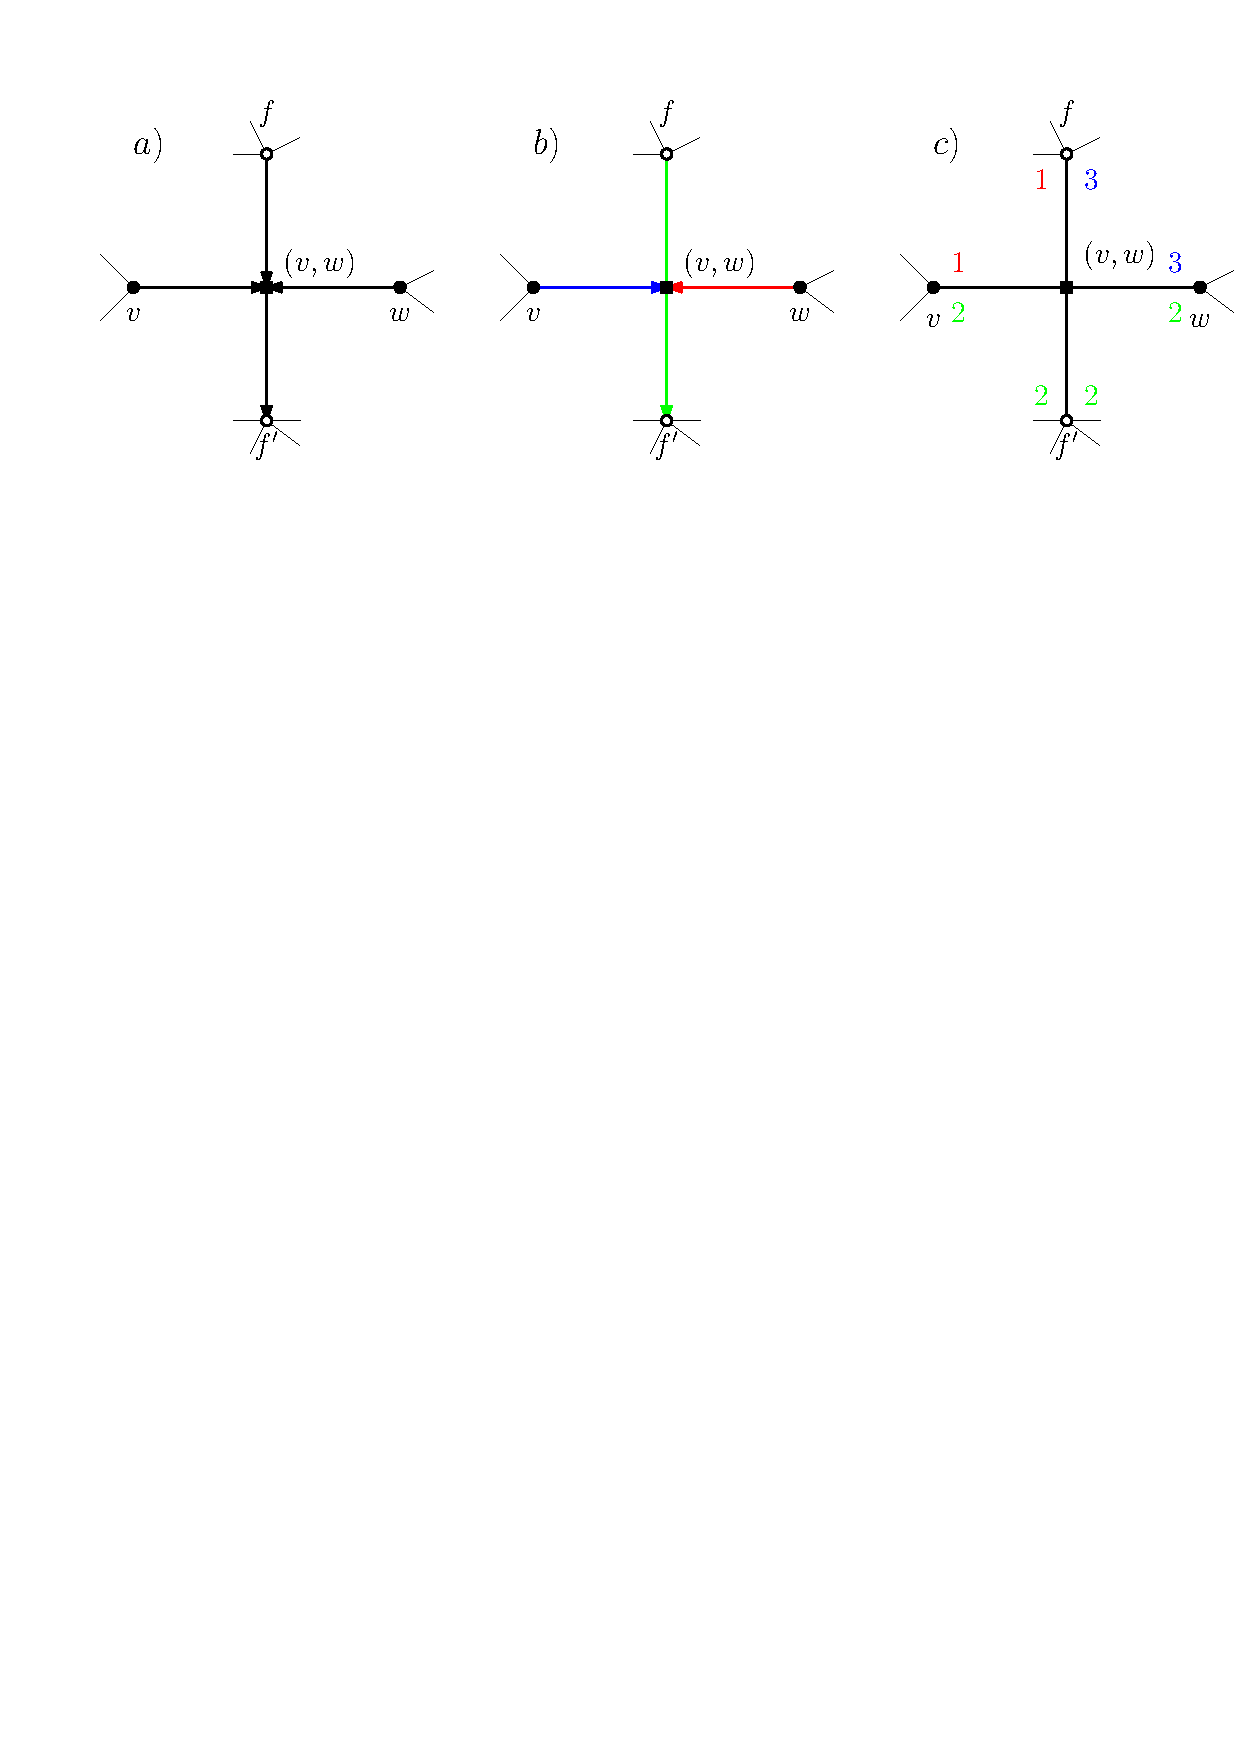
\includegraphics[width=1\textwidth]{alpha_bij.pdf}
  	\caption{a) Eine $\alpha_s$-Orientierung um eine innere Kante von $G$. b) Teile der korrespondierenden Schnyder Woods auf $G$ und $G^*$. c) Die induzierten Label, die für $G$ und $G^*$ gleich sind.}
	\label{alpha_bij_graph}
\end{figure}

Betrachten wir zuerst den \textbf{Schnyder-Fluss}. Dieser wird Fluss von Typ 1, also von Quelle 1 zu Senke 1 sein. Für einen Schnyder-Pfad, der durch einen Knoten $v$ führt, hat sich nichts geändert. Der in der Abbildung \ref{combined_face_sketch} eingezeichnete Schnyder-Pfad, der durch das innere Gebiet $f$ führt, passiert davor einen extra Knoten, wir nennen ihn \textit{kleines Quadrat}. Das kleine Quadrat soll gewährleisten, dass von Seite des Gebietes aus (also von jeder adjazenten Kante) entweder ein Schnyder-Pfad oder ein Ecken-Pfad in $f$ mündet. Zuletzt fügen wir, wie oben, von jedem inneren Gebiet eine Kante mit Kapazität $|f|-3$ zu Senke 1 ein. Somit kodiert hier eine ganzzahlige Lösung, genau wie zuvor in Netzwerk \ref{net_schnyder}, einen Schnyder Wood auf $G$.

\begin{figure}[h]
	\centering
  	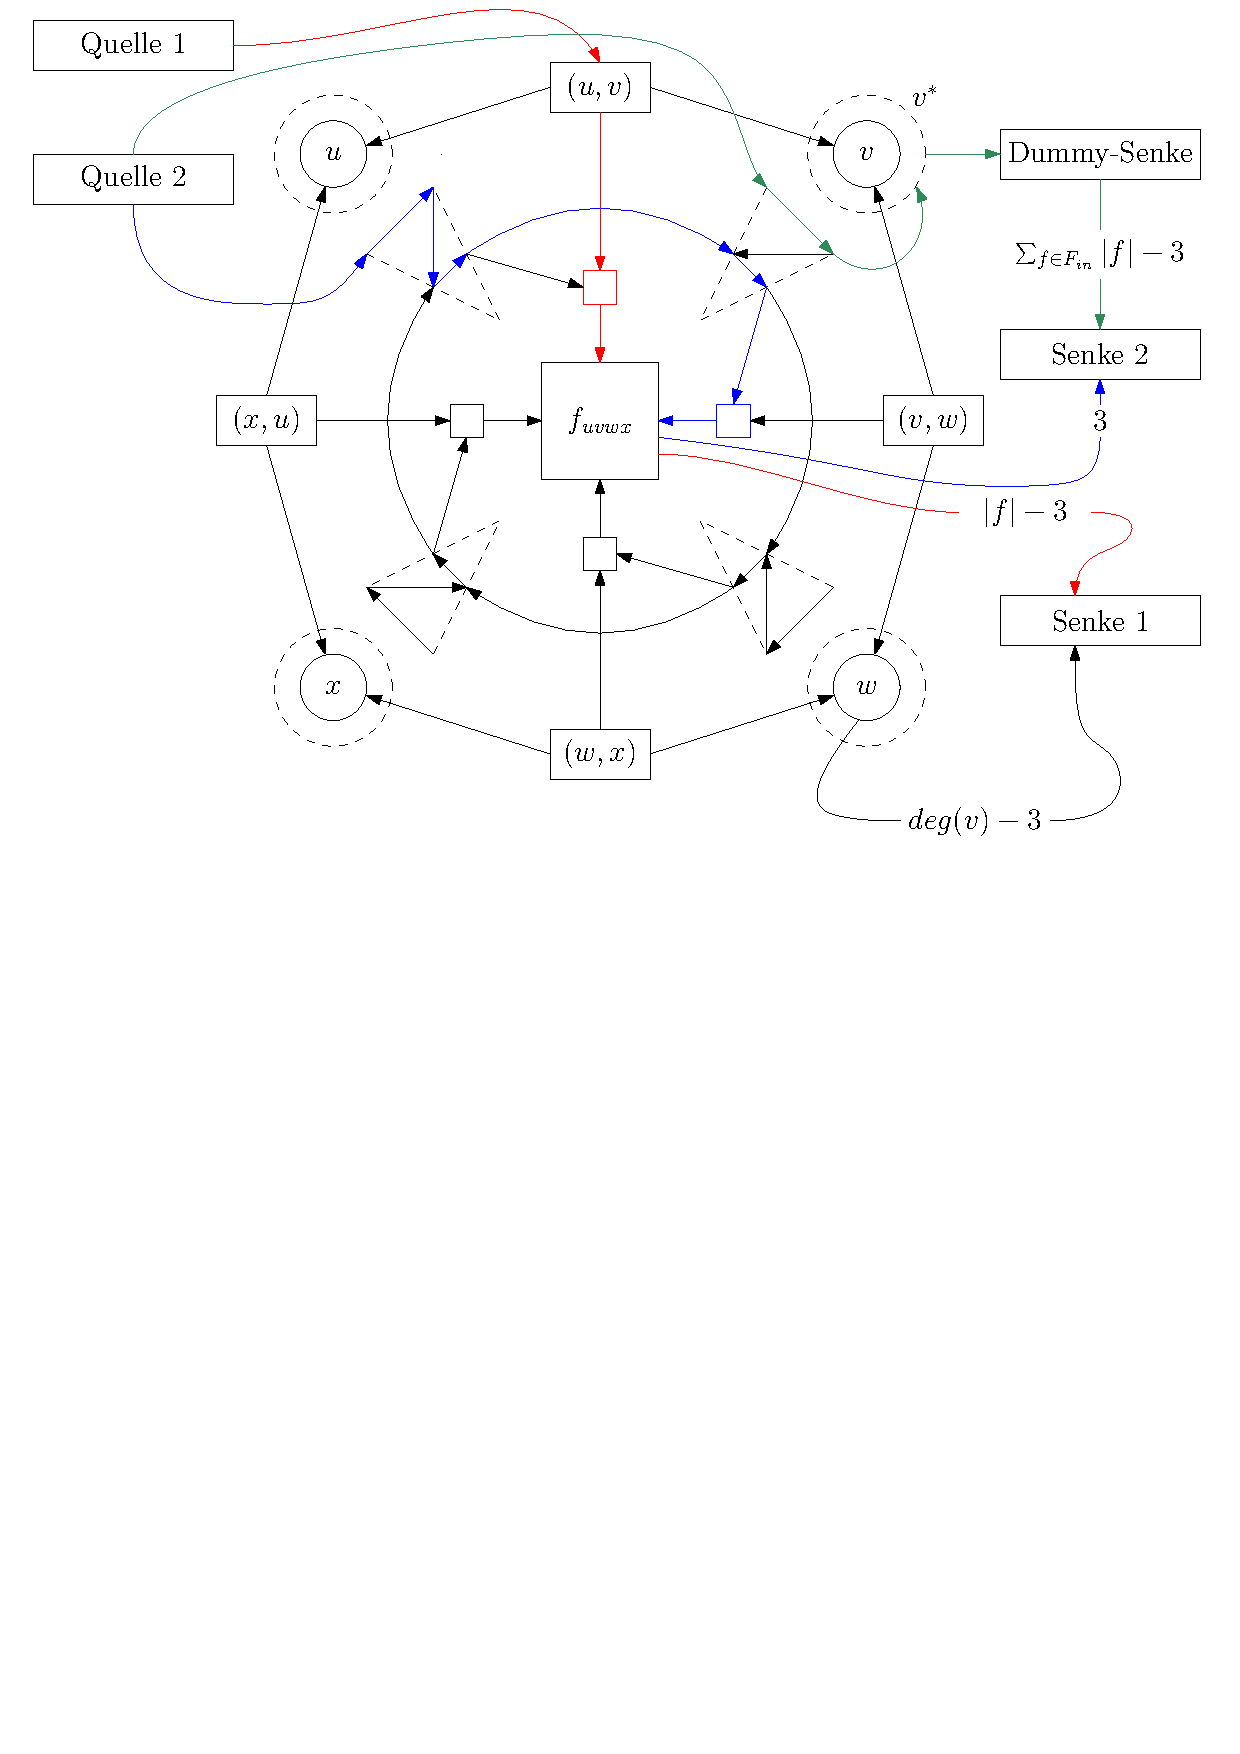
\includegraphics[width=0.95\textwidth]{combined_face_sketch.pdf}
  	\caption{Eine Skizze des kombinierten Netzwerkes auf einem inneren Gebiet mit $|f| = 4$. Beispielhaft sind ein Schnyder-Pfad (rot), ein Ecken-Pfad (blau) und ein Zuweisungs-Pfad (grün) eingezeichnet. }
	\label{combined_face_sketch}
\end{figure}

Kommen wir nun zum \textbf{FAA-Fluss}, also Fluss von Typ 2. Für einen Winkelknoten $(f,v)$ aus Netzwerk \ref{net_faa} erstellen wir ein Winkeldreieck aus vier Knoten und drei Kanten in $\mathcal{N}_G$ (vergleiche Abbildung \ref{combined_face_sketch}). Betrachten wir zuerst den im FAA-Fluss enthaltenen \textbf{Zuweisungs-Fluss}. Von Quelle 2 geht, genau wie in Netzwerk \ref{net_faa}, eine Kante zu jedem inneren Winkeldreieck $(f,v)$. Ein Zuweisungs-Pfad benutzt nur die erste Kante in einem Winkeldreieck und verlässt es über einen zusätzlich zu $v$ eingefügten Dummy-Knoten $v^*$. Von jedem $v^*$ geht eine Kante mit Kapazität 1 zu einer vorgeschobenen Dummy-Senke. Von dieser fügen wir eine Kante mit Kapazität $\sum_{f \in F_{in}} |f|-3$ zu Senke 2 ein, wie in Abbildung \ref{dummy_sink} illustriert. Die Dummy-Knoten $v^*$ sorgen dafür, dass jeder Knoten im FAA nur einmal zugewiesen werden kann, ohne in Konflikt mit dem Schnyder-Fluss zu kommen. Die eingeschobene Dummy-Senke beschränkt die Anzahl der insgesamt zugewiesenen Knoten, genau wie im zuvor konstruierten FAA-Fluss, auf $\sum_{f \in F_{in}} |f|-3$.

Es bleibt der \textbf{Ecken-Fluss}. Ein Ecken-Pfad betritt das Netzwerk durch ein Winkeldreieck $(f,v)$ und muss, bevor er das Gebiet verlässt, ein vom Schnyder-Fluss ungenutztes kleines Quadrat passieren. Die zweite und dritte Kante in jedem Winkeldreieck gewährleisten, dass nicht immer das nächste kleine Quadrat genutzt werden muss. Falls dies von Schnyder-Fluss besetzt ist und der nächste Winkel zugewiesen wird, kann ein Ecken-Pfad den nächsten Winkel passieren (wie in Abbildung \ref{combined_face_sketch}). Die erste Kante, die von sowohl Zuweisungs-, als auch Ecken-Pfaden genutzt werden kann, sorgt im Falle einer ganzzahligen Lösung für eine eindeutige Beschriftung (als Ecke oder Zuweisung). Wie zuvor existieren auch hier Kanten von jedem inneren Gebiet zu Senke 2 mit Kapazität drei.

\begin{figure}
	\centering
  	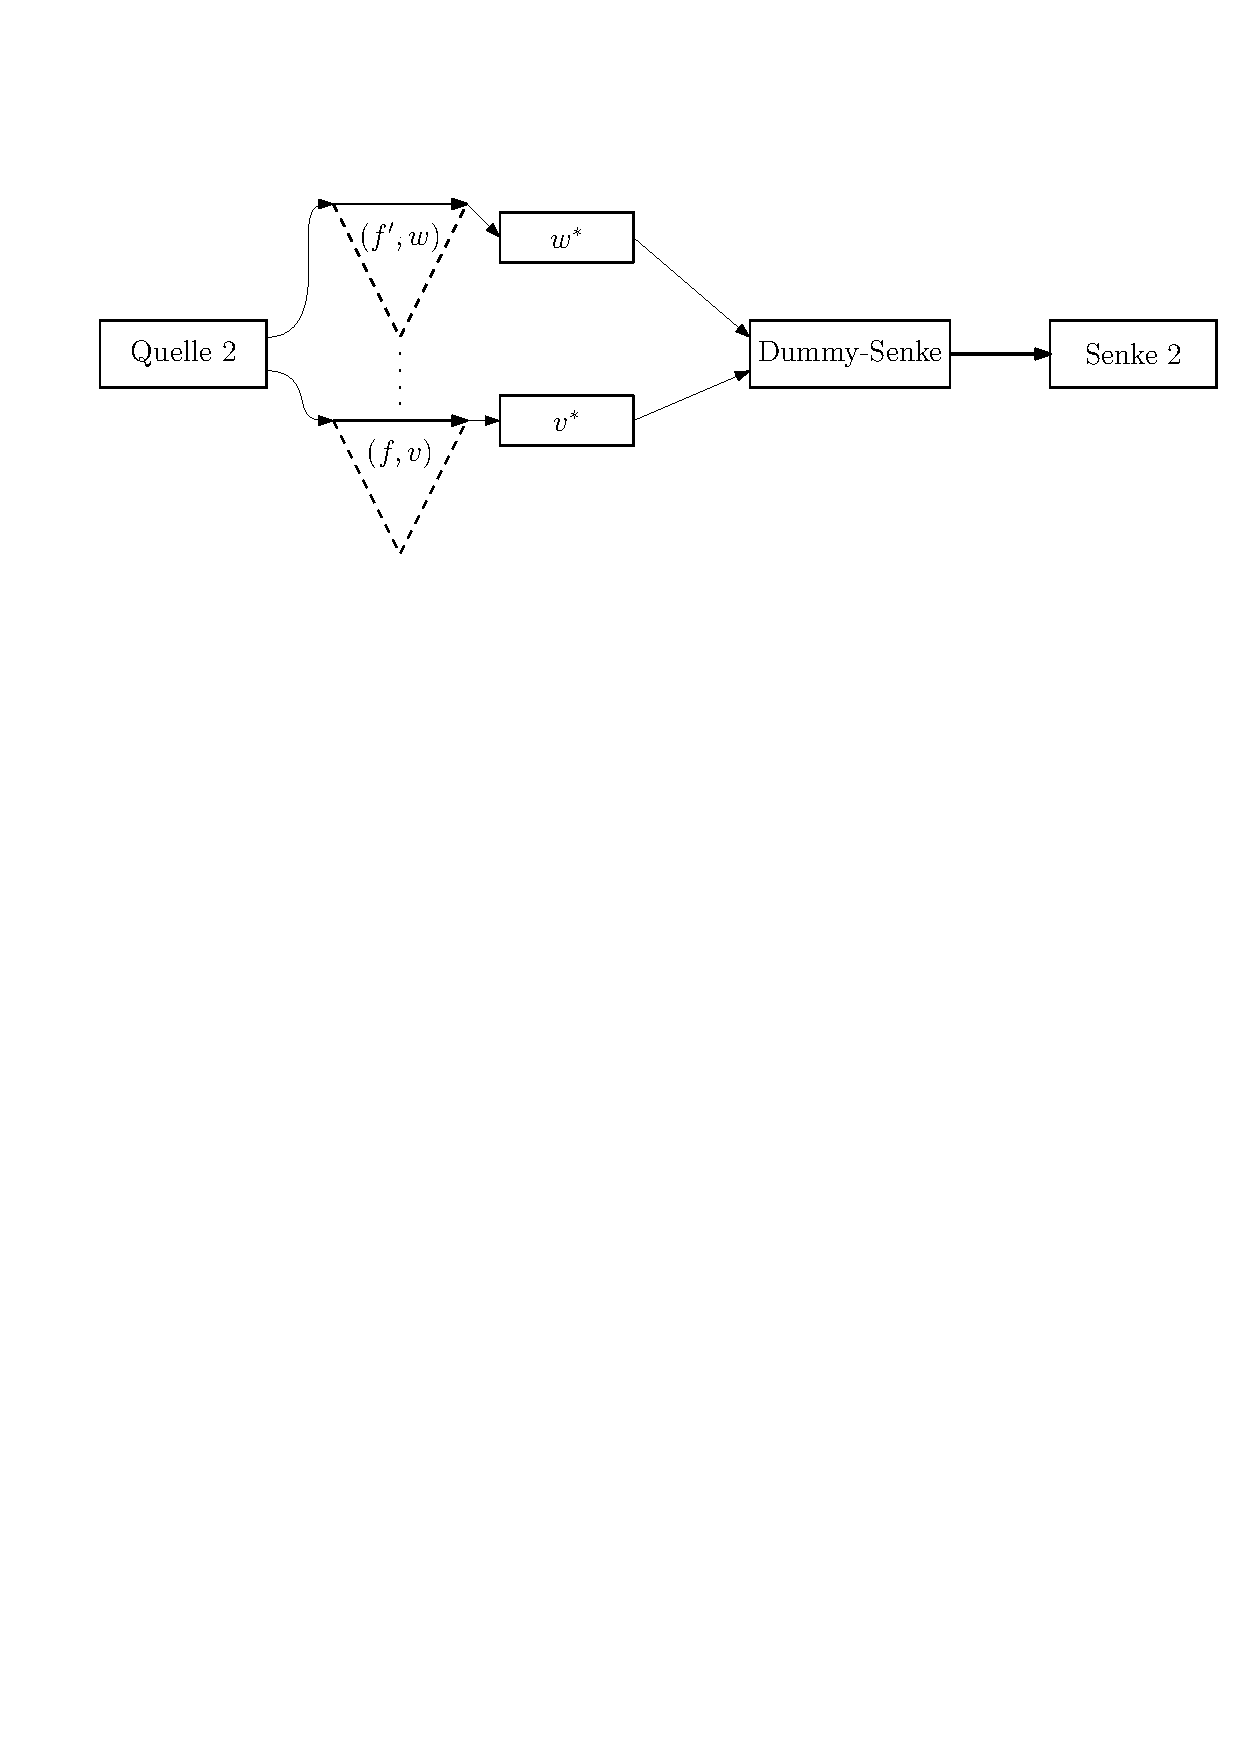
\includegraphics[width=0.85\textwidth]{dummy_sink.pdf}
  	\caption{Der Zuweisungsfluss durch die Winkel, Dummy-Knoten und die zusätzliche Kante vor Senke 2. Die Kante rechts hat Kapazität $\sum_{f \in F_{in}} |f|-3$ und alle anderen Kapazität 1.}
	\label{dummy_sink}
\end{figure}

Die Bedarfe der beiden Flüsse $\varphi_s$ bzw. $\varphi_F$ haben sich nicht verändert. Beide entsprechen jeweils den Bedarfen der oben konstruierten Netzwerke. So kann, mit den gleichen Argumenten wie oben, ein Schnyder Wood und ein FAA kodiert werden. Jedes Gebiet benötigt genau drei Ecken und $|f|-3$ zugewiesene Knoten und je ein Schnyder-Pfad führt durch jede innere Kante, $|E_{in}|$. Hier seien wieder $E_{in}$ die inneren Kanten und $F_{in}$ die inneren Gebiete von $G$. Fassen wir noch einmal zusammen.

\begin{network}[SLTR]\label{net_sltr}
Bei $\mathcal{N}_G$ handelt es sich um ein gerichtetes Netzwerk, das auf Basis eines ebenen intern-3-zusammenhängenden Graphen $G$ mit Aufhängungen $a_1,a_2,a_3$ erstellt wird, um eine SLTR von $G$ zu finden. Ein Ausschnitt um ein inneres Gebiet ist in Abbildung \ref{combined_face_sketch} dargestellt.
	\begin{itemize}
	\item $\mathcal{N}_G$ hat zwei Quellen $s_1,s_2$ und zwei Senken $t_1,t_2$
	\item Es werden Knoten der folgenden Typen in $\mathcal{N}_G$ erzeugt:
		\begin{itemize}
		\item Knoten $e$ für jede innere Kante $e \in E_{in}$
		\item Knoten $v$ für jeden $v \in V$ und Dummy-Knoten $v^*$ für jeden $v \in V_{in}$
		\item Knoten für jedes innere Gebiet $f \in F_{in}$.
		\item $|f|$ kleine Quadrate $q$ um jedes innere Gebiet $f$
		\item Vier Knoten $w_i=(f,v)_i$, mit $i\in\{1,\ldots,4\}$, für jeden inneren Winkel
		\item eine Dummy-Senke $t_d$
		\end{itemize}
	\item Es werden gerichtete Kanten der folgenden Typen in $\mathcal{N}_G$ erzeugt:
		\begin{itemize}
		\item $(s_1,e)$ von Quelle 1 zu jeder inneren Kante mit $c\big(s_1,e\big) = 1$
		\item $(e,v_1),(e,v_2)$ von jeder inneren Kante zu den Endknoten mit $c\big(e,v_i\big) = 1$
		\item $(e,q)$ von inneren Kanten zu adjazenten kleinen Quadraten mit $c\big(e,q\big) = 1$
		\item $(q,f)$ einem kleinen Quadraten zu seinem inneren Gebiet mit $c\big(q,f\big) = 1$
		\item $(f,t_1)$ von den inneren Gebieten zur Senke 1 mit $c\big(f,t_1\big) = |f|-3$
		\item $(a_i,t_1)$ von den Aufhängungen zur Senke 1 mit $c\big(a_i,t\big) = \text{deg}(a_i)-2$
		\item $(v,t_1)$ von den restlichen Knoten zur Senke 1 mit $c\big(v,t\big) = \text{deg}(v)-3$		
		\item $(s_2,w_1)$ von Quelle 2 zu jedem inneren Winkel mit $c\big(s_2,w_1\big) = 1$
		\item $(w_1,w_2),(w_2,w_3),(w_3,w_4)$ in jedem inneren Winkel mit $c\big(w_i,w_{i+1}\big) = 1$
		\item $(w_2,v*)$ von jedem inneren Winkel zum Dummy-Knoten mit $c\big(w_2,v^*\big) = 1$
		\item $(w_4,q)$ von inneren Winkeln zum nächsten kleinen Quadrat mit $c\big(w_4,q\big) = 1$
		\item $(w_4,w'_3)$ von einem inneren Winkeln zum Nächsten mit $c\big(w_4,w'_3\big) = 1$
		\item $(v^*,t_d)$ von den Dummy-Knoten zur Dummy-Senke mit $c\big(v^*,t_d\big) = 1$
		\item $(t_d,t_2)$ von der Dummy-Senke zu Senke 2 mit $c\big(t_d,t_2\big) = \sum_{f \in F_{in}}|f|-3$
		\end{itemize}
	\item $\mathcal{N}_S$ hat Bedarfe $d_1=|E_{in}|$ und $d_2 = \sum_{f \in F_{in}}|f|$
	\item [$\Rightarrow$] Ein zulässiger ganzzahliger Fluss $\varphi = (\varphi_1,\varphi_2)$ existiert. $\Leftrightarrow$ Es existiert ein SLTR  auf $G$.
	\end{itemize}
\end{network}	

Bevor wir in Theorem \ref{theo_algo} zeigen, dass eine ganzzahlige Lösung $\varphi=(\varphi_1,\varphi_2)$ auch wirklich ein Ecken kompatibles Paar kodiert, wollen wir noch ein Paar weitere Beobachtungen festhalten. Nehmen wir also an, es existiert ein ganzzahliger zulässiger Fluss $\varphi$ auf $\mathcal{N}_G$, dann gilt für diesen:
\begin{itemize}
\item [A2] Jede äußere Kante $(w_1,w_2)$ in einem Winkel-Dreieck ist ausgelastet, sie wird entweder von einem Ecken- oder Zuweisungs-Pfad genutzt.
\item [A3] Jede Kante von einem kleinen Quadrat zu einem inneren Gebiet $f$ ist ausgelastet, sie wird entweder von einem Schnyder- oder Ecken-Pfad genutzt.
\item [A4] Ein inneres Gebiet $f$ mit $|f|=3$ kann nicht von Zuweisungs- bzw. Schnyder-Pfaden genutzt werden.
\end{itemize}

Wir wollen diese Beobachtungen kurz begründen. Für jede mögliche ganzzahlige Lösung $\varphi$ gilt $$|\varphi|=|\varphi_1|+|\varphi_2| = |E_{in}| + \sum_{f \in F_{in}} |f|.$$
Da es genau $\sum_{f \in F_{in}} |f|$ innere Winkel gibt und der FAA-Fluss $\mathcal{N}_G$ nur durch diese betreten kann, ergibt sich A2. Punkt A3 wird aus Gleichung \ref{eq_sat} weiter unten folgen. Durch ein inneres Gebiet $f$ müssen drei Ecken-Pfade laufen und im Fall $|f|=3$ führt dies zu A4, da in den Winkeln kein Platz für Zuweisungs-Pfade ist und keine freien kleinen Quadrate für Schnyder-Pfade existieren.

\begin{theorem}\label{theo_algo}
Sei $G$ ein intern-3-zusammenhängender Graph mit gegebenen Aufhängungen $\{a_1,a_2,a_3\}$, dann existiert eine SLTR von $G$ genau dann, wenn ein ganzzahliger zulässiger Fluss $\varphi=(\varphi_1,\varphi_2)$ auf $\mathcal{N}_G$ existiert.
\end{theorem}

\begin{proof}[Beweis von Theorem \ref{theo_algo}]
Sei $G$ ein intern-3-zusammenhängender Graph mit Aufhängungen $\{a_1,a_2,a_3\}$ und $\varphi=(\varphi_1,\varphi_2)$ sei ein ganzzahliger zulässiger Fluss auf $\mathcal{N}_G$. Im ersten Schritt konstruieren wir einen Schnyder-Wood $\sigma$ und ein FAA $\phi$ aus $\varphi$, um dann zu zeigen, dass sie ein Ecken kompatibles Paar bilden. Für einen zulässigen Fluss müssen die Bedarfe erfüllt werden. Es gilt somit $|\varphi_1| =  |E_{in}|$ und $|\varphi_2| = \sum_{f \in F_{in}} |f|$. In der nächsten Gleichung bezeichne $f_{aus}$ das äußere Gebiet.
\begin{equation}\label{eq_sat}
\begin{split}
|\varphi_1| + |\varphi_2| & = \sum_{f \in F_{in}} (|f|-3) + 3|F_{in}| + |E_{in}|\\
		& = \sum_{f \in F_{in}} (|f|-3) + 2|E| -|V| - 1 + 2|F| - |f_{aus}|\\
		& = \sum_{f \in F_{in}} (|f|-3) + \sum_{v \in V} (\text{deg}(v)-3) + 2|V| + 2|F| - 1 - |f_{aus}|\\
		& = \sum_{f \in F_{in}} (|f|-3) + \sum_{v \in V} (\text{deg}(v)-3) + 2|E| + 3 - |f_{aus}|\\
		& = \underbrace{\sum_{f \in F_{in}}(|f|-3)  }_{\text{\parbox{8em}{Dummy-Senke zu Senke 2}}} + \underbrace{\sum_{v \in V} (\text{deg}(v)-3) +3 }_{\text{\parbox{10em}{Kapazität Senke 2 von den Knoten.}}} +\underbrace{\sum_{f \in F_{in}}(|f|-3) + 3|F_{in}|}_{\text{\parbox{12em}{Kanten von den Quadraten zu den inneren Gebieten}}}
\end{split}
\end{equation}

Die beiden Terme in der rechten unteren Klammer entsprechen den Kapazitäten von den inneren Gebieten zu Senke 1 und Senke 2. Somit sind alle Kanten zu den Senken ausgelastet. Die Kanten von den kleinen Quadraten zu den inneren Gebieten sind ebenfalls ausgelastet. Diese sind die einzigen Kanten in $\mathcal{N}_G$, die sowohl von $\varphi_1$ als auch $\varphi_2$ genutzt werden können. Kapazität eins und Ganzzahligkeit von $\varphi$ impliziert somit A3.

Beginnen wir mit $\varphi_1$, um einen Schnyder Wood, oder genauer eine $\alpha_s$-Orientierung, zu erhalten. Es gilt $|\varphi_1| = |E_{in}|$, und somit führt durch jede innere Kante ein Schnyder-Pfad. Dieser gibt uns die nach außen gerichtete Kante in $\alpha_s$. Es bleibt zu zeigen, dass für jedes innere Gebiet und jeden Knoten die Bedingungen aus Theorem \ref{alpha_bij} für eine $\alpha_s$-Orientierung eingehalten werden. Da alle Kanten von den Knoten zu Senke 1 ausgelastet sind, folgt, dass durch jeden inneren Knoten $v$ genau $\text{deg}(v)-3$ Schnyder-Pfade führen. Somit ergeben die leeren Einkanten von $v$ in $\mathcal{N}_G$ die drei Auskanten für $\alpha_s$. Für eine Aufhängung $a_i$ folgt analog, dass die beiden ungenutzten Einkanten zusammen mit der Halbkante ins äußere Gebiet, die Bedingungen der $\alpha_s$-Orientierung erfüllen. Es bleibt zu zeigen, dass durch jedes innere Gebiet $|f|-3$ Schnyder-Pfade führen. Der restliche Schnyder-Fluss mit Stärke $|E_{in}| - \sum_{v \in V} (\text{deg}(v)-3)$ muss durch die inneren Gebiete führen und aus der ersten und letzten Zeile von Gleichung \ref{eq_sat} folgt $$|E_{in}| - \sum_{v \in V} (\text{deg}(v)-3) = \sum_{f \in F_{in}} (|f|-3).$$
Somit führen $|f|-3$ Schnyder-Pfade durch jedes innere Gebiet und wir können die $\alpha_s$-Orientierung vervollständigen und erhalten einen Schnyder Wood $\sigma$ auf $G$.

Betrachten wir nun $\varphi_2$, also den FAA-Fluss. Nach A4 sind alle äußeren Kanten in den Winkeln ausgelastet. Falls diese nun in jedem inneren Gebiet von drei Ecken-Pfaden und $|f|-3$ Zuweisungs-Pfaden genutzt werden, können wir ein FAA konstruieren. Da alle Kanten zu Senke 2 ausgelastet sind, führen $\sum_{f \in F_{in}} (|f|-3)$ Pfade durch die Dummy-Senke. Somit werden auch $\sum_{f \in F_{in}} (|f|-3)$ Knoten inneren Gebieten zugewiesen. Indem wir diese Pfade zurückverfolgen und überprüfen, aus welchem Gebiet der Zuweisungs-Pfad einen Dummy-Knoten betritt, erhalten wir die Zuweisungen. Es bleibt zu zeigen, dass jedem Gebiet genau $|f|-3$ Knoten zugewiesen werden. Dies gilt genau dann, wenn durch jedes Gebiet drei Ecken-Pfade laufen. Da die Kanten von den inneren Gebieten zu Senke 2 ausgelastet sind, können wir also aus $\varphi_2$ ein FAA $\phi$ für $G$ konstruieren.

Nun müssen wir zeigen, dass das Schnyder Labeling $\sigma$ und das FAA $\phi$ ein Ecken kompatibles Paar ergeben. Die Bedingung K1, dass beide die gleichen Aufhängungen nutzen, folgt sofort aus der Konstruktion von $\mathcal{N}_G$. Es bleibt K2, also betrachten wir ein Teilnetzwerk (wie in Abbildung \ref{combined_face_sketch}) um ein inneres Gebiet $f$. Die drei Ecken-Pfade können keine der $|f|-3$ kleinen Quadrate nutzen, die schon von Schnyder-Fluss okkupiert werden. Die drei übrigen kleinen Quadrate nennen wir \textit{verfügbar}. Ausgehend von $f$ folgen wir den Ecken-Pfaden rückwärts zu den verfügbaren kleinen Quadraten. Wenn wir das Quadrat verlassen, gelangen wir zur dritten Kante eines Winkeldreiecks (entgegen dem Uhrzeigersinn). Nun verlassen wir das Gebiet entweder über diesen Winkel oder bewegen uns weiter (entgegen dem Uhrzeigersinn) zum nächsten Winkeldreieck. Wir zeigen in Behauptung \ref{claim1}, dass dies nur dann geschieht, wenn das kleine Quadrat zwischen diesen nicht verfügbar ist. Also betritt zwischen jeweils zwei verfügbaren kleinen Quadraten ein Ecken-Pfad das Gebiet und die Winkel haben nach A1 unterschiedliche Label in $\sigma$.

\begin{claim}\label{claim1}
Seien $Q_1,Q_2$ und $Q_3$ im Uhrzeigersinn die drei verfügbaren kleinen Quadrate um ein inneres Gebiet $f$. Dann existiert ein Ecken-Pfad, welcher das Netzwerk über $Q_i$ verlässt. Dieser betritt es in einem Winkel zwischen, im Uhrzeigersinn, $Q_{i-1}$ und $Q_i$.
\end{claim}

\begin{figure}
	\centering
  	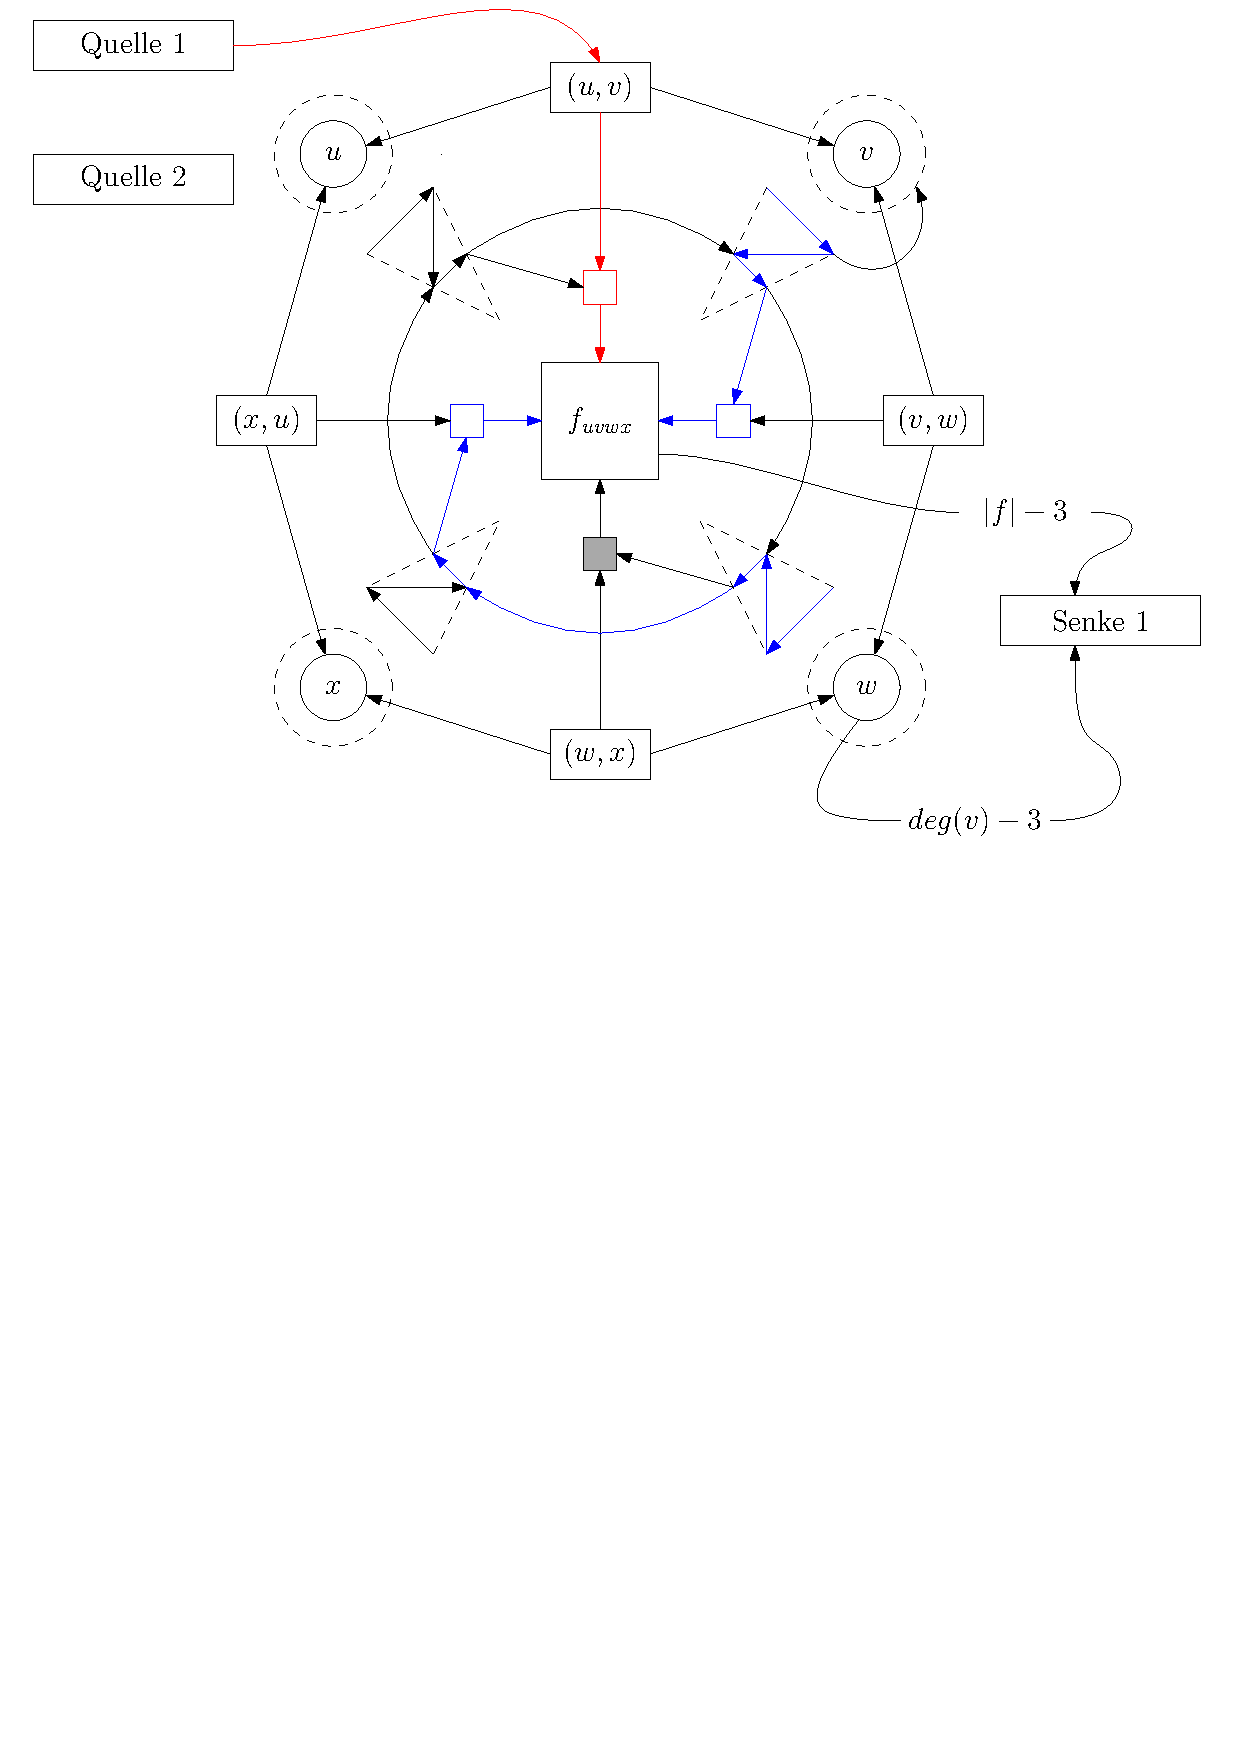
\includegraphics[width=0.9\textwidth]{combined_face_skip.pdf}
  	\caption{Das untere \textit{verfügbare} kleine Quadrat (grau) wird vom Ecken-Fluss (blau) übersprungen und kann nicht mehr ausgelastet werden.}
	\label{combined_face_skip}
\end{figure}

Angenommen dies ist nicht der Fall und nehmen wir ohne Beschränkung der Allgemeinheit an, dass der Ecken-Pfad $P_e$ das Gebiet durch $Q_3$ verlässt. Der Winkel, über den $P_e$ das Teilnetzwerk um das innere Gebiet betritt, liegt also nicht zwischen $Q_2$ und $Q_3$ (vergleiche Abbildung \ref{combined_face_skip}). Angenommen er liegt zwischen $Q_1$ und $Q_2$. Betrachte das letzte Winkeldreieck vor $Q_2$. Nach unserer Annahme ist die innere Kante dieses Dreiecks von $P_e$ ausgelastet. Somit kann kein Ecken-Fluss zu $Q_2$ gelangen und wir erhalten einen Widerspruch, da alle kleinen Quadrate entweder von Ecken- oder von Schnyder-Fluss genutzt werden müssen. Mit dem gleichen Argument kann $P_e$ das Teilnetzwerk nicht zwischen $Q_3$ und $Q_1$ betreten. Somit ist Behauptung \ref{claim1} wahr.

\begin{claim}\label{claim_angle}
Alle Winkel zwischen zwei aufeinander folgenden verfügbaren kleinen Quadraten haben die selben Label im Schnyder Labeling $\sigma$.
\end{claim}

Diese Behauptung folgt aus A1. Die Winkel links und rechts von einem kleinen Quadrat, dass von einem Schnyder-Pfad genutzt wird, haben das gleiche Label in $\sigma$, da diese den Einkanten in $\alpha_s$ entsprechen. Die Auskanten entsprechen den verfügbaren kleinen Quadraten, und hier ändern sich die Label. Diese beiden Behauptungen zusammen zeigen, dass jede Ecke aus $\phi$ ein anderes Label in $\sigma$ hat. Somit handelt es sich um ein Ecken kompatibles Paar $(\sigma,\phi)$.

Wir haben die Rückrichtung gezeigt. Nehmen wir also an, dass eine SLTR für $G$ existiert. Wir müssen nun einen zulässigen ganzzahligen Fluss $\varphi=(\varphi_1,\varphi_2)$ auf $\mathcal{N}_G$ konstruieren, der die SLTR kodiert. Nach Theorem \ref{theo_ccc} existiert ein Ecken kompatibles Paar $(\sigma,\phi)$ aus einem Schnyder Labeling $\sigma$ und einem FAA $\phi$, das zu diesem SLTR passt. Betrachte die zu $\sigma$ gehörige $\alpha_s$-Orientierung.

Wir beginnen mit einem leeren, wie oben konstruierten Netzwerk $\mathcal{N}_G$ und werden nun Schritt für Schritt einen zulässigen Fluss $\varphi$ konstruieren. Zuerst fügen wir für jeden zugewiesenen Winkel einen Pfad von Quelle 2, über die äußere Kante des Winkeldreiecks, den zugehörigen Dummy-Knoten und die Dummy-Senke hin zu Senke 2 ein. Es kommen somit $\sum_{f \in F_{in}}|f|-3$ Einheiten Fluss hinzu und die Kante von der Dummy-Senke zu Senke 2 wird ausgelastet. 

Als nächsten fügen wir den Schnyder-Fluss hinzu, der die $\alpha_s$-Orientierung kodiert. Zuerst von Quelle 1 zu jedem inneren Kanten-Knoten $e$, dann von den inneren Kanten entweder über ein kleines Quadrat in ein angrenzendes Gebiet oder zu einem benachbarten Knoten, je nachdem, wohin die Auskante von $e$ in $\alpha_s$ zeigt. Als Konsequent müssen wir auch die Kanten von den inneren Knoten und inneren Gebieten zu Senke 1 sättigen.

Zuletzt fügen wir den Ecken-Fluss ein. Ein Ecken-Pfad $P_e$ beginnt in Quelle 1, nutzt das zugehörige Winkeldreieck (diese sind noch frei) und verlässt das Gebiet über das im Uhrzeigersinn nächste verfügbare kleine Quadrat. Das dieser Weg frei ist folgt wieder aus Behauptung \ref{claim_angle}. Es sind somit alle Kanten zu den Senken ausgelastet, ohne die Kapazität einer Kante zu überschreiten. Somit haben wir einen zulässigen ganzzahligen Fluss konstruiert, der eine SLTR kodiert. Damit ist der Beweis abgeschlossen.
\end{proof}

\begin{remark}
Wir können die Quellen und Senken von Netzwerk \ref{net_sltr} nicht vereinen und trotzdem gewährleisten, dass eine zulässige ganzzahlige Lösung ein SLTR kodiert. In Netzwerk \ref{net_sltr} verlieren wir so die Kontrolle über die Menge von Zuweisungs-Fluss der durch jedes innere Gebiet fließt. Wir erhalten mit einer zulässigen ganzzahligen Lösung also nicht mehr zwangsläufig ein FAA.

Wir können das Netzwerk leicht abwandeln, um sicher zu stellen, dass eine ganzzahlige Lösung immer eine FAA und einen Schnyder Wood induziert, doch dann geht uns die Kontrolle über die Ecken-Kompatibilität verloren.
\end{remark}

\section{Nicht-ganzzahlige Flüsse auf $\mathcal{N}_G$}\label{sec_non_int}

Wir werden uns zum Abschluss des Kapitels mit der von Aerts und Felsner offen gelassenen Frage beschäftigen, ob die Erkennung von Graphen mit einer SLTR in P liegt -- ob also polynominelle deterministische Algorithmen für die Entscheidung existieren, ob für einen gegebenen Graphen eine SLTR existiert. Wie in Abschnitt \ref{dir_multi_flow} erwähnt, impliziert eine nicht ganzzahlige Lösung für ein Gerichtetes-Multi-Fluss-Problem auf einem Graphen mit $n\geq 2$ Paaren von Quellen und Senken im Allgemeinen nicht die Existenz einer ganzzahligen Lösung. Und nach Theorem \ref{np_hard} ist die Berechnung einer ganzzahligen Lösung NP-schwer. Die experimentellen Ergebnisse aus Kapitel \ref{the_program} lassen jedoch die Möglichkeit offen, dass wir für das betrachtete Netzwerk $\mathcal{N}_G$ die folgende Vermutung beweisen können.

\begin{conjecture}\label{int_conj}
Sei $\tilde{\varphi}=(\tilde{\varphi_1},\tilde{\varphi_2})$ ein nicht ganzzahliger zulässiger Fluss auf $\mathcal{N}_G$, dann existiert auch ein ganzzahliger zulässiger Fluss $\varphi$ und wir können in polynomieller Zeit ein Gutes-FAA aus $\tilde{\varphi_2}$ konstruieren.
\end{conjecture}

\begin{remark}
Wenn wir nicht darauf bestehen, dass ein berechneter zulässiger Fluss auf $\mathcal{N}_G$ ganzzahlig ist, dann lässt sich ein zulässiger Fluss wie in Abschnitt \ref{dir_multi_flow} erwähnt durch lineare Programmierung in polynomineller Zeit finden und das Entscheidungsproblem, ob ein Graph eine SLTR hat, läge so in P.
\end{remark}

Es ist uns noch nicht gelungen, einen Beweis von Vermutung \ref{int_conj} zu finden. Wir werden zuerst einen Weg besprechen, um ein FAA aus einer nicht-ganzzahligen Lösung zu konstruieren. Wir Vermuten, dass es sich bei diesem FAA um ein Gutes-FAA handelt. Danach werden wir zwei mögliche Beweisansätze betrachten. Um die Argumentation einfacher zu gestalten, werden wir das Zwei-Fluss-Problem manchmal als Drei-Fluss Problem, mit einer Lösung $\varphi=(\varphi_s,\varphi_e,\varphi_z)$ betrachten, indem wir Schnyder-, Ecken-, und Zuweisungs-Fluss eigene Typen und somit Quellen und Senken zuweisen.

\begin{proposition}
Sei $\mathcal{N}^*_G$ ein Netzwerk bei dem wir Schnyder-, Ecken-, und Zuweisungs-Fluss jeweils eigene Quellen und Senken zuweisen und das sonst analog zu $\mathcal{N}_G$ konstruiert wird. Dann existiert ein zulässiger (ganzzahliger) Fluss $\varphi^*=(\varphi^*_s,\varphi^*_e,\varphi^*_z)$ auf $\mathcal{N}^*_G$ genau dann, wenn ein zulässiger (ganzzahliger) Fluss $\varphi=(\varphi_1,\varphi_2)$ auf 
$\mathcal{N}_G$ existiert.
\end{proposition}

\begin{proof}
Wir müssen den FAA-Fluss aus $\mathcal{N}_G$ in zwei Typen aufteilen. In der Bemerkung nach Proposition \ref{prop_net_faa} haben wir schon einen Weg beschrieben, dies zu tun. In $\mathcal{N}_G^*$ existieren jeweils von der Ecken- und Zuweisungs-Quelle Kanten zum ersten Knoten der Winkeldreiecke. Die Winkel-Senke ist Senke 2 und wir trennen die Dummy-Senke von Senke 2 und machen sie zur Zuweisungs-Senke. Sonst sind $\mathcal{N}_G$ und $\mathcal{N}^*_G$ gleich. Die Bedarfe werden entsprechend aufgeteilt. Somit sind die einzigen von Ecken- und Zuweisungs-Fluss gemeinsam nutzbaren Kanten die ersten Kanten in den Winkeldreiecken. Für den Schnyder-Fluss verändert sich nichts.

Angenommen wir haben einen zulässigen (ganzzahligen) Fluss $\varphi^*=(\varphi^*_s,\varphi^*_e,\varphi^*_z)$ auf $\mathcal{N}_G^*$, dann induziert $(\varphi_s,\varphi_e+\varphi_z)$ auch einen zulässigen (ganzzahligen) Fluss auf $\mathcal{N}_G$. Sei nun $\varphi=(\varphi_1,\varphi_2)$ ein zulässiger (ganzzahliger) Fluss auf $\mathcal{N}_G$. Dann gilt $\varphi_1 = \varphi^*_s$. Wir müssen also $\varphi_2$ aufteilen. Ein (ganzzahliger) FAA-Pfad, der ein Winkeldreieck betritt, verlässt es entweder durch einen Dummy-Knoten oder führt weiter in das Gebiet. Wir können $\varphi_2$ somit in $\varphi_e^*$ und $\varphi_z^*$ aufteilen. Es bleibt zu zeigen, dass die Bedarfe erfüllt sind. In $\mathcal{N}_G$ führt eine Kante mit Kapazität drei von jedem inneren Gebiet zu Senke 2, die von $\varphi_2$ gesättigt ist. Dieser Anteil des FAA-Flusses wird nach Konstruktion zu $\varphi_e^*$. Somit bleibt in jedem inneren Gebiet $|f|-3$ Zuweisungs-Fluss. Die Bedarfe sind somit erfüllt. Die Ecken-Kompatibilität ergibt sich wie im Beweis zu Theorem \ref{theo_algo}.
\end{proof}

Insbesondere gilt dieser Zusammenhang für eine beliebige Kombination von Ecken-, Schnyder- und Zuweisungs-Fluss zu zwei Flüssen, und wir müssen die Netzwerke nur leicht abwandeln. Die Flüsse lassen sich aber auch nach diesen Veränderung, von einem auf ein anderes Netzwerk übertragen.

\begin{proposition}\label{choose_types}
Für jede beliebige Kombination von Schnyder-, Ecken- und Zu\-weis\-ungs-Fluss zu zwei Flüssen auf einem zu $\mathcal{N}^*_G$ analog konstruierten Netzwerk existiert ein zulässiger (ganzzahliger) Fluss $\varphi$ genau dann, wenn ein zulässiger (ganzzahliger) Fluss $\varphi^*=(\varphi^*_s,\varphi^*_e,\varphi^*_z)$ auf $\mathcal{N}^*_G$ existiert. Ein zulässiger (ganzzahliger) Fluss $\varphi$ existiert also insbesondere genau dann, wenn eine zulässige (ganzzahlige) Lösung für eine beliebige andere Kombination der Flüsse existiert.
\end{proposition}

\begin{proof}
Wie wir einen zulässigen (ganzzahligen) Fluss $\varphi$ aus $\varphi^*$ konstruieren ist klar. Betrachten wir denn Fall, dass wir Schnyder- und Zu\-weis\-ungs-Fluss zu $\varphi_1$ kombinieren. Wir fügen zwischen der Zuweisungs-Quelle und den Winkeldreiecken für jedes innere Gebiet einen zusätzlichen Knoten ein. Zu diesen Knoten führt eine Kante mit Kapazität $|f|-3$ von der Zuweisungs-Quelle und Kanten zu den Winkeln der entsprechenden inneren Gebiete mit Kapazität 1 (vergleiche Abbildung \ref{pic_faa_choice}). Sei nun $\varphi=(\varphi_1,\varphi_2)$ ein zulässiger (ganzzahliger) Fluss. Für den Zuweisungs-Fluss $\varphi_2=\varphi_z$ verändert sich nichts. $\varphi_2$ lässt in jedem inneren Gebiet genau Platz für Ecken-Pfade mit Kapazität 3 frei. Wir können einen Pfad in $\varphi_1$ nun Zuweisungs-Fluss oder Schnyder-Fluss zuweisen, indem wir überprüfen, ob er das kleine Quadrat von einem Kanten-Knoten oder einem Winkeldreieck aus betritt. Durch jedes innere Gebiet führen Ecken-Pfade mit Auslastung 3 und somit Schnyder-Pfade mit Auslastung $|f|-3$. Die Ecken-Kompatibilität zeigt man wieder analog zum Beweis von Theorem \ref{theo_algo}. Die Kombination aus Schnyder- und Ecken-Fluss folgt nach Aerts und Felsner \cite{af15}. Hier reicht wieder der Beutel im Zuweisungs-Fluss, um die Korrektheit des Netzwerkes zu erhalten.
\end{proof}

\begin{proposition}\label{claim_non_int}
Angenommen es existiert eine zulässige nicht-ganzzahlige Lösung $\tilde{\varphi}$ auf $\mathcal{N}_G$ und $\mathcal{N}_G$ lässt keine ganzzahlige Lösung zu, dann müssen die drei Flüsse $\tilde{\varphi}_e, \tilde{\varphi}_z$ und $\tilde{\varphi}_s$ alle nicht-ganzzahlig sein. Insbesondere muss mindestens ein Teilnetzwerk um ein inneres Gebiet existieren, auf dem alle drei Flüsse nicht-ganzzahlig sind.
\end{proposition}

\begin{proof}
Sei der Ecken-Fluss $\tilde{\varphi}_e$ ganzzahlig. Dann existieren auf $\mathcal{N}_G$ keine Kanten die von zwei Flusstypen genutzt werden, da sich $\tilde{\varphi}_z$ und $\tilde{\varphi}_s$ nach Konstruktion keine Kanten teilen können. Somit erhalten wir nach Theorem \ref{theo_int_flow} für alle drei Flüsse eine ganzzahlige Lösung. Wir können somit annehmen, dass $\tilde{\varphi}_e$ nicht-ganzzahlig ist. Wir definieren nun den Schnyder-Fluss als Fluss von Typ 1 und den Zuweisungs-Fluss als Typ 2 und werden den Ecken-Fluss lokal entweder dem einen oder dem anderen zuordnen. 

Betrachten wir ein Teilnetzwerk um inneres Gebiet, auf dem $\tilde{\varphi}_s$ ganzzahlig ist, dann ordnen wir lokal den Ecken-Fluss Typ 2 zu. Wir behalten so trotzdem die Kontrolle über die Anzahl der zugewiesenen Winkel in diesem Gebiet und die Ecken-Kompatibilität, falls wir eine neue Lösung berechnen. Analog ordnen wir den Ecken-Fluss Typ 1 zu, falls der Zuweisungs-Fluss ganzzahlig ist. Somit existieren keine Kanten, die in unserer Lösung von beiden Flüssen gleichzeitig genutzt werden. Nach Theorem \ref{theo_int_flow} existieren zulässige ganzzahlige Flüsse von Typ 1 und Typ 2. Dies liefert einen zulässigen ganzzahligen Fluss auf $\mathcal{N}_G$, was ein Widerspruch zur Annahme ist, dass dieser nicht existieren kann.
\end{proof}

Betrachten wir zunächst den zweiten Teil von Vermutung \ref{int_conj}. Die nächste Proposition liefert eine Methode, um aus einem nicht ganzzahligen zulässigen Fluss ein FAA zu konstruieren.

\begin{proposition}\label{lem_faa}
Sei $\tilde{\varphi}$ ein nicht ganzzahliger zulässiger Fluss auf $\mathcal{N}_G$ und sei $W$ die Menge der vom Zuweisungsfluss $\tilde{\varphi}_z$ genutzten inneren Winkel von $G$. Dann existiert eine Teilmenge $\phi\subseteq W$, sodass aus jedem Gebiet $f$ genau $|f|-3$ Winkel in $\phi$ enthalten sind und in der jeder Knoten $v$ höchstens einmal vorkommt. $\phi$ ist also ein FAA auf $G$.
\end{proposition}

\begin{proof}
Sei $\tilde{\varphi}$ ein nicht ganzzahliger zulässiger Fluss auf $\mathcal{N}_G$. Wir definieren das gerichtete Netzwerk $\mathcal{F}_z$ mit Quelle $s$ und Senke $t$, einem Beutel $B_f$ für jedes innere Gebiet $f$, einem Knoten für jeden inneren Winkel $(f,v) \in W$ und einem Knoten für jeden Dummy-Knoten. Zuerst fügen wir Kanten mit Kapazität $|f|-3$ von der Quelle zu jedem Beutel ein. Dann folgen Kanten von den Beuteln $B_f$ zu den Winkeln von $f$, von den Winkeln $(f,v)$ zu den Dummy-Knoten $v^*$ und zuletzt eine Kante von jedem Dummy-Knoten zu Senke, jeweils mit Kapazität 1. Die Kanten zu den Beuteln bilden einen Schnitt mit Kapazität $\sum_{f \in F_{in}}(|f|-3)$ und $\tilde{\varphi}_z$ induziert einen zulässigen nicht-ganzzahligen Fluss $\varphi^*$ auf $\mathcal{F}_z$. Die Stärke eines maximalen $s$-$t$-Fluss in $\mathcal{F}_z$ ist somit $\sum_{f \in F_{in}}(|f|-3)$. Nach Theorem \ref{theo_int_flow} existiert also ein ganzzahliger zulässiger Fluss $\varphi$ auf $\mathcal{F}_z$, mit $|\varphi| = |\varphi^*| = |\tilde{\varphi}_z| = \sum_{f \in F_{in}}(|f|-3).$

\begin{figure}
	\centering
  	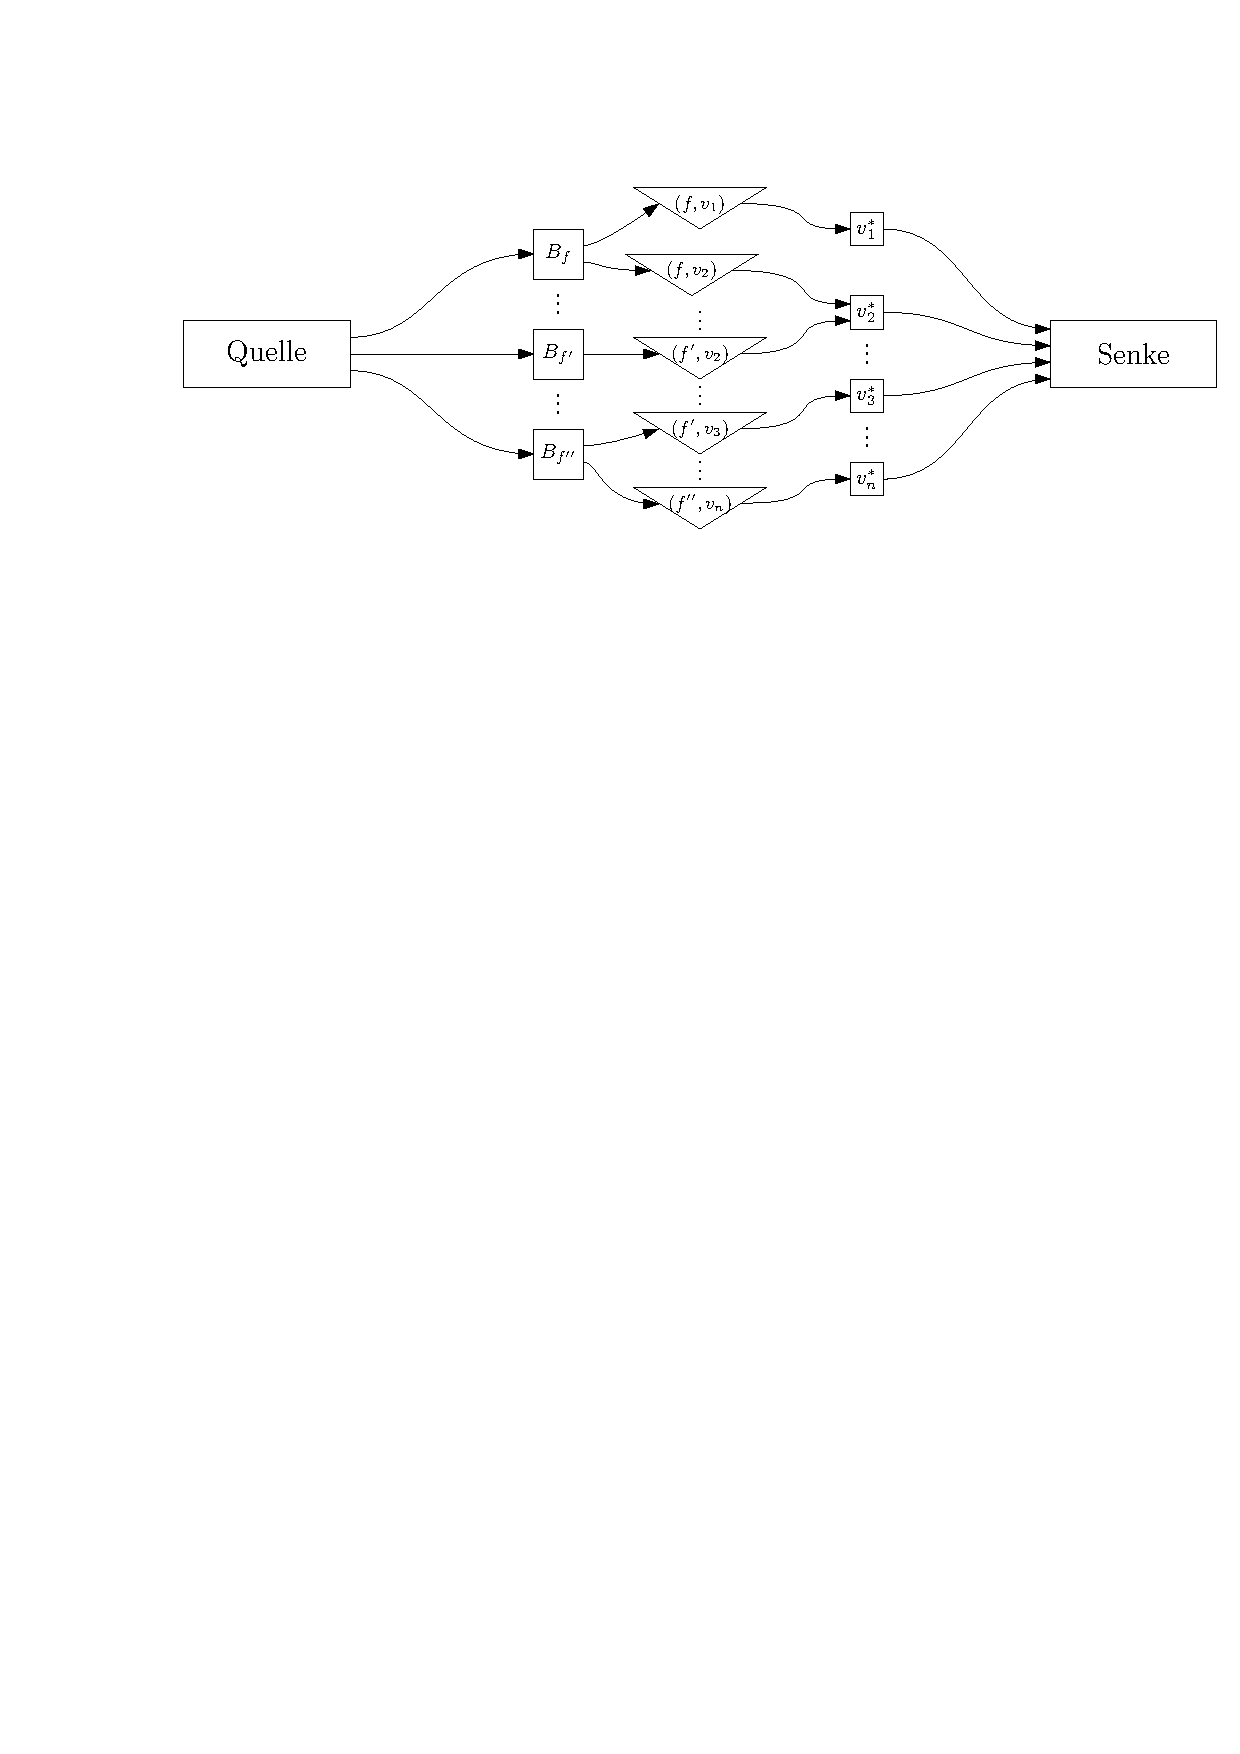
\includegraphics[width=0.9\textwidth]{lem_faa_choice.pdf}
  	\caption{Skizze des Netzwerkes $\mathcal{F}_z$. Die Kanten von der Quelle zu einem Beutel $B_f$ hat Kapazität $|f|-3$ und alle anderen haben Kapazität 1.}
	\label{pic_faa_choice}
\end{figure}

Der Fluss $\varphi$ weißt nun jedem inneren Gebiet $f$ genau $|f|-3$ Winkel zu und jeder Knoten $v$ kann nur einmal zugewiesen werden. Wenn wir noch die Knoten hinzunehmen, die per Konstruktion von $\mathcal{N}_G$ dem äußeren Gebiet zugewiesen sind, dann erhalten wir ein FAA auf $G$.
\end{proof}

Wenn wir zeigen könnten, dass ein wie in Proposition \ref{lem_faa} konstruiertes $\phi$ ein Gutes-FAA ist, folgt Vermutung \ref{int_conj}, da die Existenz eines Guten-FAAs $\phi$ nach Theorem \ref{theo_algo} auch die Existenz eines ganzzahligen zulässigen Flusses $\varphi$ für $\mathcal{N}_G$ impliziert. Die Ergebnisse aus Kapitel \ref{the_program} legen nahe, dass es sich um ein Gutes-FAA handelt. Formulieren wir dies als eine zweite Vermutung.

\begin{conjecture}\label{faa_conj}
Ein wie in Proposition \ref{lem_faa}, aus einem zulässigen Fluss auf $\mathcal{N}_G$ konstruiertes FAA $\phi$ ist ein Gutes-FAA von $G$ und induziert somit eine SLTR.
\end{conjecture}

\begin{figure}[b]
\centering
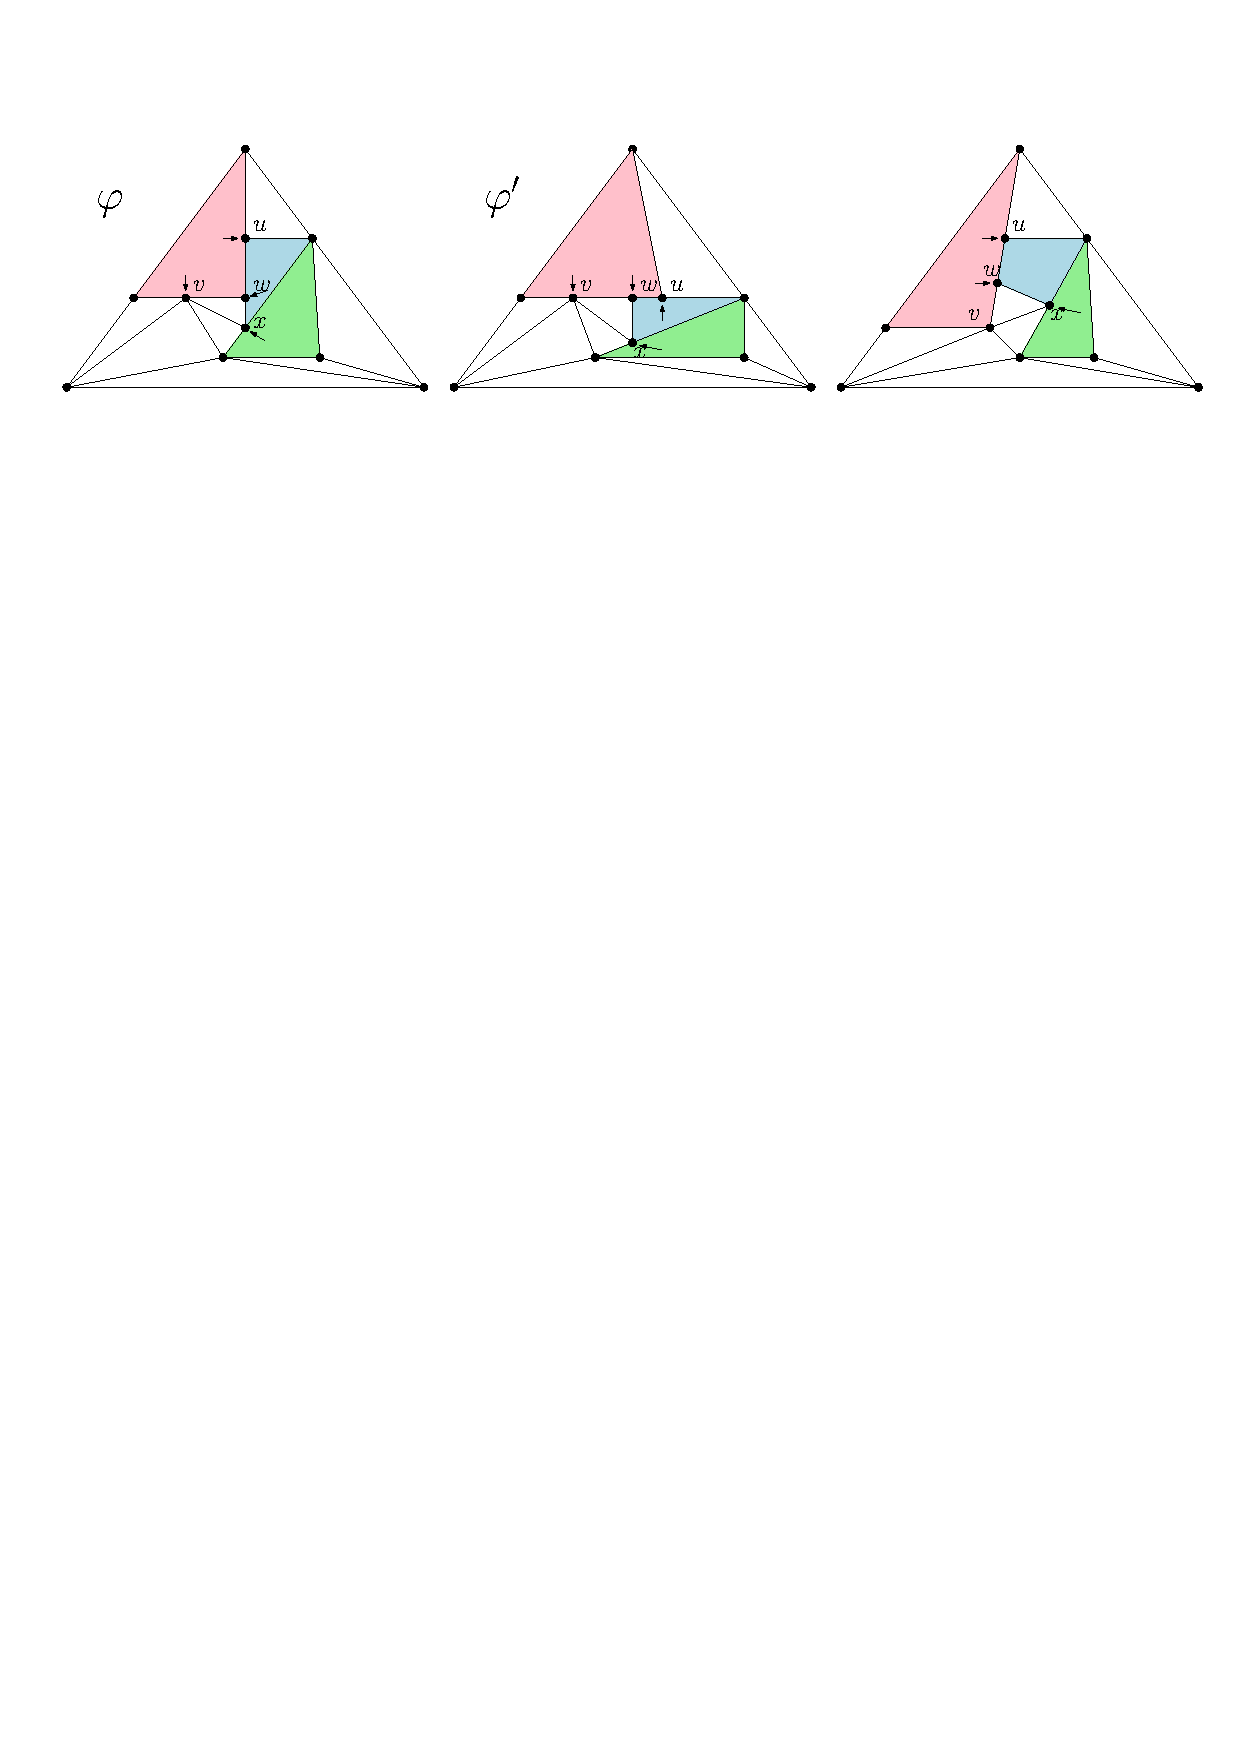
\includegraphics[width=1\textwidth]{lem_faa_choice_ex.pdf}
\caption{Bei der Auswahl der Winkel aus W ist Vorsicht geboten.}
\label{lem_faa_choice_ex}
\end{figure}


\begin{example}
Es ist nicht möglich mit beliebigen Winkeln aus $W$ zu beginnen und Schritt für Schritt für jedes Gebiet $|f|-3$ Winkel wählen. Betrachte den planaren Graphen $G$ aus Abbildung \ref{lem_faa_choice_ex}. Die beiden SLTRs auf der linken Seite haben dieselben Aufhängungen, implizieren jedoch andere FAAs und somit auch andere zulässige ganzzahlige Flüsse auf $\mathcal{N}_G$. Seien $\varphi$ und $\varphi'$ diese Flüsse und $f_{r},f_{g}$ und $f_b$ die drei eingefärbten Gebiete. Betrachten wir die Zuweisungs-Flüsse $\varphi_z$ und $\varphi'_z$. Dann gilt $$|\varphi_z(f_r,v)|=|\varphi_z(f_r,u)|=|\varphi_z(f_b,w)| = |\varphi_z(f_g,x)| = 1$$
$$|\varphi_z(f_r,v)|=|\varphi_z(f_r,w)|=|\varphi_z(f_b,u)| = |\varphi_z(f_g,x)| = 1.$$
Der Fluss $\tilde{\varphi}=\frac{\varphi+\varphi'}{2}$ ist ebenfalls zulässig und es folgt:
$$|\tilde{\varphi}_z(f_r,v)|=|\tilde{\varphi}_z(f_g,x)| = 1, \text{ und } $$
$$|\tilde{\varphi}_z(f_r,w)|=|\tilde{\varphi}_z(f_r,u)| = |\tilde{\varphi}_z(f_b,w)|=|\tilde{\varphi}_z(f_b,u)| = \frac{1}{2}.$$
Somit liegen all diese Winkel in W. Wir können allerdings nicht einfach beginnen in einem Gebiet die benötigte Anzahl an Winkeln auszuwählen. In Abbildung \ref{lem_faa_choice_ex} führt dies auf der rechten Seite zu keinem FAA und somit auch zu keiner SLTR. Die Konstruktion des Netzwerkes im Beweis von Proposition \ref{lem_faa} ist somit sinnvoll.
\end{example}

\subsection{Minimale Schnitte in $\mathcal{N}_G$}

Wir wollen in diesem Abschnitt einen ersten möglichen Beweisansatz von Vermutung \ref{int_conj} besprechen. Die Idee ist, dass wir unter der Annahme, dass nur eine nicht-ganzzahlige Lösung existiert, einen minimalen Schnitt in einem Teilnetzwerk von $\mathcal{N}_G$ erzeugen, und so zu einem Widerspruch gelangen. 

Angenommen, es existiert ein Netzwerk $\mathcal{N}_G$, für das nur eine nicht ganzzahlige Lösung existiert. Sei $\tilde{\varphi}$ dieser nicht ganzzahlige zulässige Fluss und $\phi$ ein wie in Proposition \ref{lem_faa} aus $\tilde{\varphi}$ konstruiertes FAA für $G$. Sei $\varphi_z$ der eindeutige Zuweisungs-Fluss, der dieses FAA auf $\mathcal{N}_G$ kodiert und $\overline{\mathcal{N}}_G$ das Teilnetzwerk von $\mathcal{N}_G$, aus welchem alle Kanten, die von $\varphi_z$ ausgelastet sind, gelöscht wurden. Die Bedarfe sind weiterhin $|E_{in}|$ und $3|F_{in}|$ für den Schnyder- und Ecken-Fluss. Nach Proposition \ref{choose_types} können wir $\varphi_s$ und $\varphi_e$ zusammenfassen und mit $\varphi_1$ bezeichnen. Wir suchen also nach einem zulässigem ganzzahligem Fluss $\varphi_1 = \varphi_s + \varphi_e$ auf $\overline{\mathcal{N}}_G$ mit Bedarf $|E_{in}| + 3|F_{in}|$, da dann auch nach Bemerkung \ref{claim_non_int} eine ganzzahlige Lösung $(\varphi_s,\varphi_e)$ folgen würde. Wir hätten somit einen ganzzahligen Fluss auf $\mathcal{N}_G$ konstruiert, was zu einem Widerspruch führt.

Nach dem Max-Flow Min-Cut Theorem existiert ein zulässiger Fluss auf $\overline{\mathcal{N}}_G$ genau dann, wenn es keinen (Kanten-)Schnitt in $\overline{\mathcal{N}}_G$ mit Kapazität kleiner als $|E_{in}| + 3|F_{in}|$ gibt, der Quelle und Senke trennt. Bevor wir fortfahren, wollen wir einige Kantentypen aus $\mathcal{N}_G$ benennen.

\begin{itemize}
\item $E_\triangle = $ Die äußeren Kanten in den Winkeldreiecken.
\item $E_\triangledown = $ Die inneren Kanten in den Winkeldreiecken.
\item $S_* =$ Die Kanten von den Dummy-Knoten zur Dummy-Senke.
\item $V_* = $ Die Kanten von den Winkeldreiecken zu den Dummy-Knoten.
\item $E_{\to} = $ Die Kanten von Quelle 1 zu den Kanten-Knoten.
\item $F_\square = $ Die Kanten von den kleinen Quadraten zu inneren Gebieten $f$.
\item $V_{\to} = $ Die Kanten von den Knoten-Knoten zu Senke 1.
\item $e_{d} = $ Die Kante von der Dummy-Senke zu Senke 2
\end{itemize}

Sowohl $\mathcal{S}_1 = E_\triangle \cup E_{\to}$, als auch $\mathcal{S}_2 = F_\square \cup V_{\to} \cup \{e_{d}\}$ sind minimale Schnitte in $\mathcal{N}_G$. Für beide Menge gilt $|\mathcal{S}_1| = |\mathcal{S}_2| = |E_{in}| + \sum{f \in F_{in}}$ und sie trennen die Quellen ($\mathcal{S}_1$) bzw. die Senken ($\mathcal{S}_2$) vom Rest des Netzwerkes ab. Wenn wir nur von den Kanten aus $E_\triangle$, die in $\overline{\mathcal{N}}_G$ übrig sind, sprechen, schreiben wir $\overline{E}_\triangle$. Für die zu diesen korrespondierenden Kanten im Inneren ihrer Winkeldreiecke schreiben wir $\overline{E}_\triangledown$. Für die Teilmengen von $V_*$ und $S_*$ in $\overline{\mathcal{N}}_G$ schreiben wir $\overline{S}_*$ und $\overline{V}_*$. Die restlichen Mengen sind vollständig in $\overline{\mathcal{N}}_G$ enthalten.

Seien $E_z$ die von $\varphi_z$ genutzen Kanten, die wir aus $\mathcal{N}_G$ entfernen. Dann folgt $|\mathcal{S}_1 \cap E_z| = |E_\triangle \cap E_z| = |\varphi_z|$. Somit ist $\overline{\mathcal{S}}_1 = \mathcal{S}_1 \backslash E_z = \overline{E}_\triangle \cup E_\to$ ein Schnitt in $\overline{\mathcal{N}}_G$. Analog ist $\overline{\mathcal{S}}_2 = F_\square \cup V_{\to}$ ein Schnitt. Für die Kapazität von $\overline{\mathcal{S}}_1$ können wir folgern 
$$ c(\overline{\mathcal{S}}_1) = c(\overline{E}_\triangle) + c(E_\to) = c(E_\triangle) - |\varphi_z| + c(E_\to) = 3|F_{in}| + |E_{in}|,$$
und wieder folgt analog $c(\overline{\mathcal{S}}_2) = 3|F_{in}| + |E_{in}|$.

Falls es sich hierbei um minimale Schnitte handelt, dann würde dies bedeuten, dass eine ganzzahlige Lösung für $\overline{\mathcal{N}}_G$ existiert, mit deren Hilfe wir, zusammen mit $\varphi_z$, eine ganzzahlige zulässige Lösung für $\mathcal{N}_G$ konstruieren könnten, was wiederum ein Widerspruch zu unserer Annahme wäre. Es muss also einen kleineren Schnitt $\mathcal{S}_{min}$, mit $|\mathcal{S}_{min}| \leq 3|F_{in}| + |E_{in}| - 1$, geben. 

\begin{remark}
Falls wir nach demselben Schema diejenigen Kanten aus $\mathcal{N}_G$ entfernen, welche von einem Zuweisungs-Fluss gesättigt sind, der einem FAA entspricht, das keine SLTR induziert, dann muss so ein minimaler Schnitt $\mathcal{S}_{min}$ existieren. Sonst würde ein Widerspruch zu Theorem \ref{theo_ccc} entstehen.
\end{remark}

Falls Vermutung \ref{faa_conj} korrekt ist, dann könnte so ein Schnitt nicht existieren. Nehmen wir jedoch für den Moment an, dass $\mathcal{S}_{min}$ wie oben beschrieben existiert, dann können wir die folgenden Beobachtungen festhalten.

\begin{claim} \label{cut_types1}
Falls $\mathcal{S}_{min}$ existiert, dann muss auch ein minimaler Schnitt $\mathcal{S}_{min}^*$ in $\overline{\mathcal{N}}_G$ existieren, sodass er nur Kanten von einem der vier Typen $\overline{E}_\triangledown, F_\square, V_\to$ und $E_\to$ enthält.
\end{claim}

\begin{figure}
	\centering
  	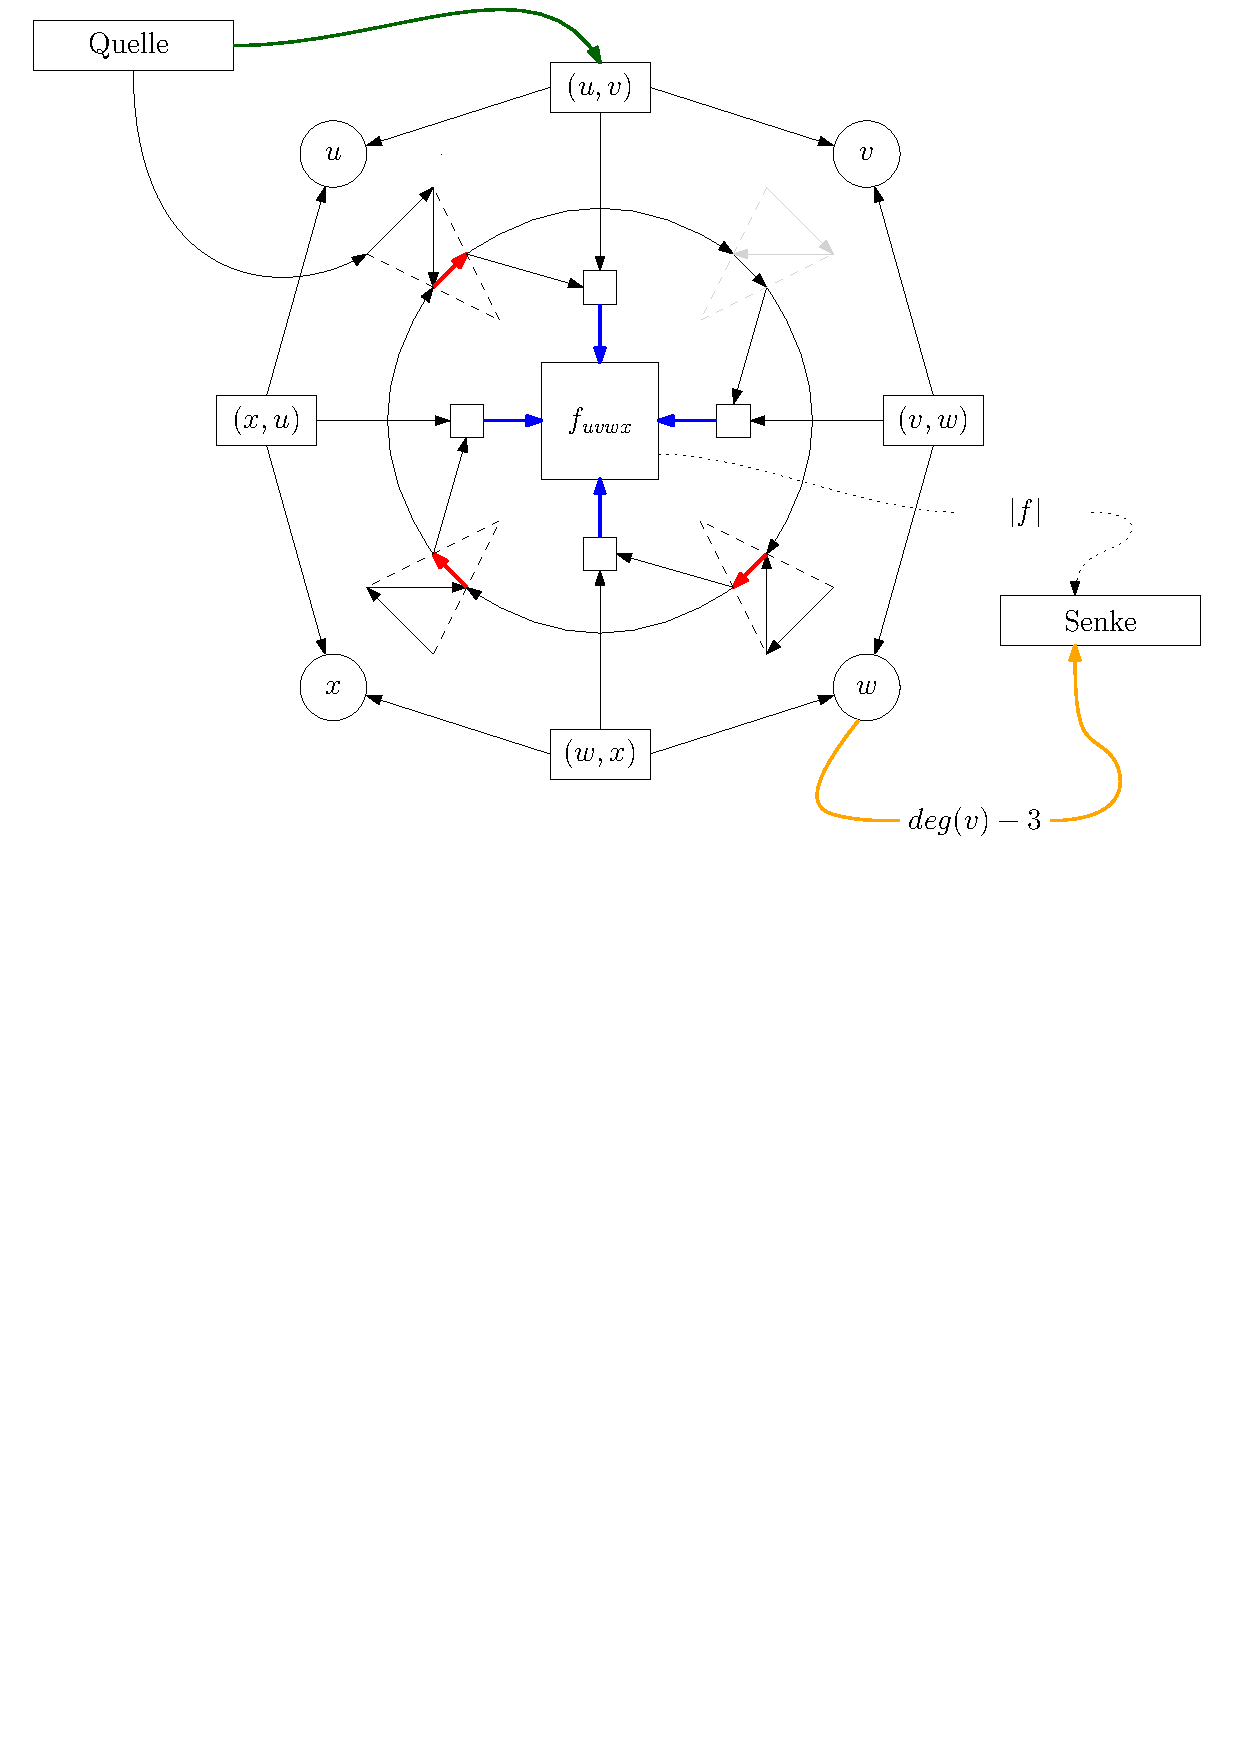
\includegraphics[width=0.8\textwidth]{face_cut.pdf}
  	\caption{Die vier Kantentypen $\overline{E}_\triangledown$ (rot), $F_\square$ (blau), $V_\to$ (orange) und $E_\to$ (grün), aus denen sich, nach Behauptungen \ref{cut_types1} und \ref{cut_types2}, ein minimaler Schnitt in $\overline{\mathcal{N}}_G$ zusammensetzen müsste.}
	\label{cut_edges}
\end{figure}

Betrachten wir die Kanten in $\mathcal{S}_{min}$. Die vier Kantentypen aus denen $\mathcal{S}_{min}^*$ bestehen soll, sind in Abbildung \ref{cut_edges} eingezeichnet. Wir werden argumentieren, dass wir Kanten, die nicht zu einer der vier Mengen gehören, eindeutig durch eine Kante aus diesen Mengen ersetzen können. Kanten auf einem Pfad von der Quelle, durch die korrespondierende Kante in $\overline{E}_\triangle$ zu einer Kante in $\overline{E}_\triangledown$, können in $\mathcal{S}_{min}^*$ durch diese ersetzen. Ebenso können Kanten zwischen zwei Winkeldreiecken, oder von einem Winkeldreieck zu einem kleinen Quadrat\footnote{Die Kante zwischen Winkeldreieck und kleinem Quadrat ließe sich ebenfalls durch die Kante aus $F_\square$ ersetzen.} in $\mathcal{S}_{min}^*$ durch die entgegen dem Uhrzeigersinn nächste Kante in $\overline{E}_\triangledown$ ersetzt werden. Kanten zwischen einem Kanten-Knoten und einem Knoten-Knoten oder einem kleinen Quadrat, können in $\mathcal{S}_{min}^*$ durch die zuvor kommende Kante aus $E_\to$ ersetzt werden. Abschließend können Kanten von einem inneren Gebiet zu Senke in $\mathcal{S}_{min}^*$ durch das Hinzufügen von allen Kanten aus $F_\square$ an diesem Gebiet ersetzt werden.

\begin{claim}\label{cut_types2}
Falls $\mathcal{S}_{min}$ existiert, dann muss auch ein minimaler Schnitt $\mathcal{S}_{min}^*$ in $\overline{\mathcal{N}}_G$ existieren, sodass er nur Kanten von einem der vier Typen $\overline{E}_\triangledown, F_\square, V_\to$ und $E_\to$ enthält. Er enthält aus jeder der Mengen $\overline{E}_\triangledown, F_\square, V_\to$ und $E_\to$ mindestens eine, aber aus keiner der Mengen alle Kanten.
\end{claim}

\begin{proof}
Falls ein solcher ein Schnitt $\mathcal{S}_{min}^*$ existiert, dann kann $\mathcal{S}_{min}^*$ nicht alle Kanten in $\overline{E}_\triangledown$ enthalten. Sonst könnten wir aus $\mathcal{S}^*_{min} \cup (E_\triangle \cap E_z)$ einen Schnitt $\mathcal{S}$ mit der gleichen Kapazität konstruieren, indem wir die Kanten $E_\triangledown \cap \mathcal{S}^*_{min}$ durch die korrespondierenden Kanten in $E_\triangle$ ersetzen. Es folgt $\mathcal{S} \supseteq\mathcal{S}_1$, was ein Widerspruch ist. Falls $\mathcal{S}_{min}^*$ jedoch keine Kante aus $\overline{E}_\triangledown$ enthält, dann muss $\mathcal{S}_{min}^*$ alle Kanten aus $F_\square$ enthalten, weil $\mathcal{S}_{min}^*$ ein Schnitt ist. Falls $\mathcal{S}_{min}^*$ alle Kanten aus $F_\square$ enthält, dann können wir annehmen, dass $\mathcal{S}_{min}^*$ auch alle Kanten aus $V_\to$ enthält. Es folgt $\mathcal{S}^*_{min} \cup \{e_d\} \supseteq \mathcal{S}_2$, was erneut ein Widerspruch ist. Angenommen $\mathcal{S}_{min}^*$ enthält keine Kante aus $F_\square$, dann muss er alle Kanten aus $\overline{E}_\triangledown$ und $E_\to$ enthalten und $\mathcal{S}^*_{min} \cup (E_\triangle \cap E_z)$ wäre erneut ein Schnitt mit Kapazität $\geq |\mathcal{S}_1|$. 

Es bleibt die Mengen $E_\to$ und $V_\to$ zu betrachten. Aus $\mathcal{S}_{min}^*\cap E_\to = \emptyset $ folgt $F_\square\subset\mathcal{S}_{min}^*$ und aus $\mathcal{S}_{min}^*\cap V_\to = \emptyset $ folgt $E_\to \subset  \mathcal{S}_{min}^*$. Im Fall $E_\to \subset  \mathcal{S}_{min}^*$ müssen um jedes innere Gebiet mindestens drei Kanten in $\mathcal{S}_{min}^*$ liegen, womit wir wieder mindestens Kardinalität $|S_1|$ erreichen. Wir betrachten als letztens $V_\to$. Hierbei ist zu beachten, dass für Knoten $v$ mit deg$(v) \leq 3$ keine Kante in $\mathcal{N}_G$ existiert. Es gelte $V_\to \subset  \mathcal{S}_{min}^*$, dann muss $\mathcal{N}_G$ noch mindestens $|E_\to|-|V_\to|$ Kanten enthalten, um den Schnyder-Fluss zu unterbrechen, was ein Widerspruch ist. Es gelte nun $\mathcal{S}_{min}^*\cap V_\to = \emptyset$. Wir benötigen erneut mindestens $|E_{in}|$ Kanten in $\mathcal{S}_{min}^*$, um den Schnyder-Fluss zu unterbrechen und wir erhalten somit einen letzten Widerspruch. Behauptung \ref{cut_types2} ist somit richtig.
\end{proof}

Schnyder- und Ecken-Fluss in $\overline{\mathcal{N}}_G$ können nur über die Kanten von Typ $E_\to, V_\to$ und $F_\square$, beziehungsweise $\overline{E}_\triangledown$ und $F_\square$, fließen. Der einzige Kantentyp, der in beiden vorkommt, ist $F_\square$. Diese Kanten wurden in Netzwerk \ref{net_sltr} eingefügt, um die Ecken-Kompatibilität zu erzwingen. Wir finden genau dann keinen ganzzahligen Fluss auf $\overline{\mathcal{N}}_G$, wenn es keinen Ecken-Kompatiblen Schnyder-Wood $\sigma$ zu dem nach Proposition \ref{lem_faa} erzeigten FAA $\phi$ gibt. Somit muss jeder zulässige Schnyder-Fluss (der einem beliebigen Schnyder Wood auf $G$ entspricht) in mindestens einem Gebiet die kleinen Quadrate so auslasten\footnote{Genauer gesagt, sprechen wir hier von den Kanten aus $F_\square$.}, dass aus mindestens einem freien Winkel keinen Ecken-Pfad führen kann. Alle kleinen Quadrate zwischen einem freien Winkel und dem im Uhrzeigersinn nächsten müssen in diesem Fall vom Schnyder-Fluss gesättigt sein. So ein kleines Quadrat ist in Abbildung \ref{combined_face_not_corner}) rot eingefärbt. 

Wir nennen eine Kante aus $F_\square$ an einem kleinen Quadrat ein \textit{blockierendes} Quadrat, falls ein zulässiger ganzzahliger Schnyder-Fluss existiert, sodass dieses kleine Quadrat das erste nach einem freien Winkel ist, der durch den Schnyder-Fluss von der Senke abgeschnitten wird.

\begin{figure}
	\centering
  	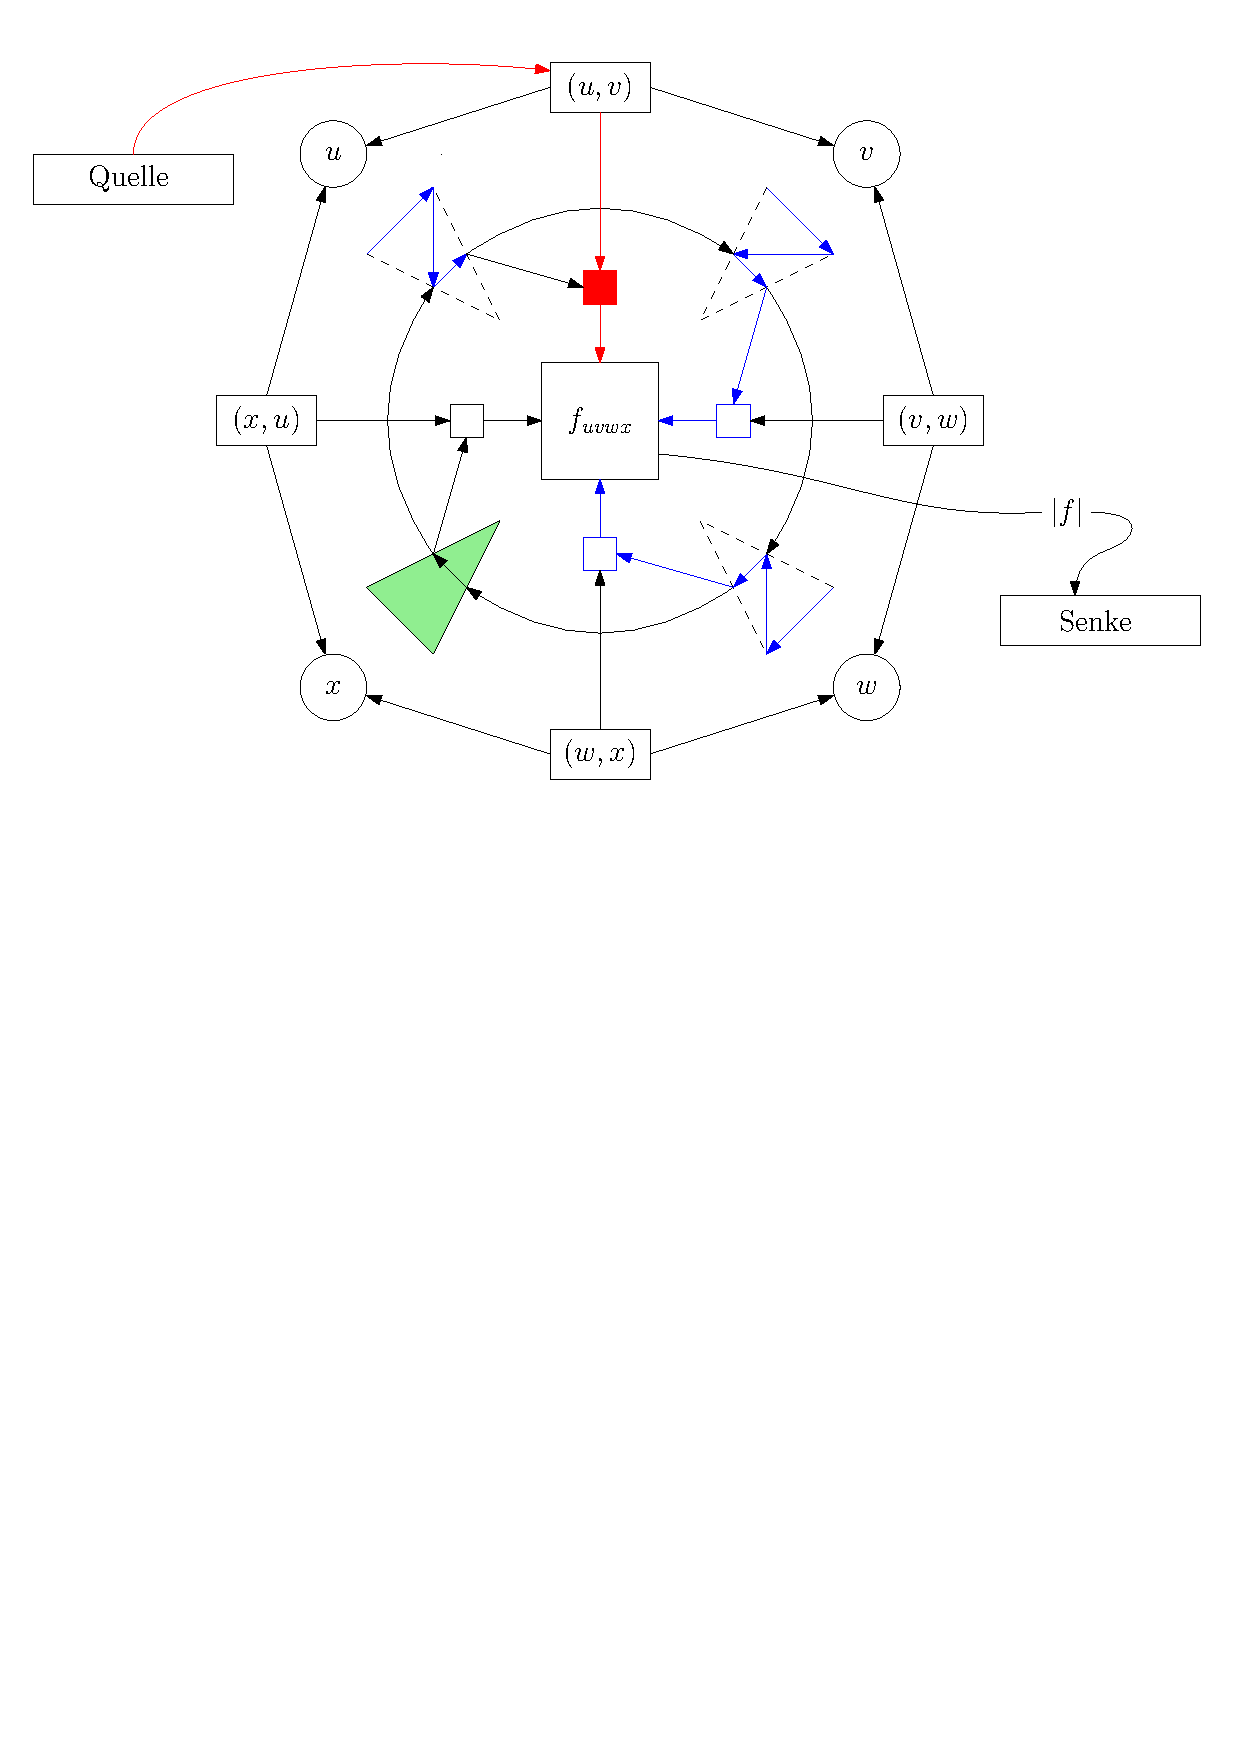
\includegraphics[width=0.7\textwidth]{combined_face_not_corner.pdf}
  	\caption{Der Schnyder-Fluss (rot) ist nicht Ecken kompatibel zum FAA $\phi$ (grün). Somit muss ein blockiertes Quadrat (hier in rot) in $\mathcal{N}_G$ existieren und durch mindestens einen freien Winkel kann kein Ecken-Pfad führen.}
	\label{combined_face_not_corner}
\end{figure}

\begin{claim}
Falls $\mathcal{S}_{min}$ existiert, dann existiert ein Schnitt $\mathcal{S}^*_{min}$ wie in Behauptung \ref{cut_types2}, welcher alle blockierenden Quadrate enthält.
\end{claim}

Falls ein blockierenden Quadrat nicht in $\mathcal{S}^*_{min}$ enthalten ist, enthält $\mathcal{S}^*_{min}$ die korrespondierenden Kanten aus $E_\to$ und die gegen den Uhrzeigersinn nächste Kante aus $E_\triangledown$. Da es sich um ein blockierendes Quadrat handelt, kann der Ecken-Fluss aus diesem Winkeldreieck nicht vorher das Gebiet verlassen. Wir können somit die Kante am Winkeldreieck in $\mathcal{S}^*_{min}$ durch das blockierende Quadrat ersetzen. \\

Uns ist es jedoch bis jetzt nicht gelungen, mit diesem Ansatz zu einem Widerspruch zu gelangen und wir beenden die Überlegungen zu minimalen Schnitten an diesem Punkt.

\subsection{Alternierende Zykel auf $\mathcal{N}_G$}

Wir werden nun einen zweiten Beweisansatz erläutern. Sei $\tilde{\varphi}=(\tilde{\varphi}_s,\tilde{\varphi}_F)$ wieder ein (nicht-ganzzahliger) zulässiger Fluss auf $\mathcal{N}_G$. Wir können diesen Fluss in Pfade aufteilen. Diese Pfade werden bei einer nicht-ganzzahligen Lösung zumindest zum Teil fraktional sein\footnote{Der Fluss der auf so einem Pfad von der Quelle zur Senke gelangt ist nicht-ganzzahlig.}. Die Idee, die wir verfolgen wollen, ist, dass wir auf Teilmengen von Kanten in $\mathcal{N}_G$ den Fluss vertauschen können, und wieder einen zulässigen Fluss erhalten. Das Ziel ist es, einen zulässigen Fluss zu konstruieren, der weniger oder gar keinen fraktionalen Anteil mehr hat.

Die formelle Definition dieses Ansatzes erfolgt nach einer Methode für $\alpha_s$-Orientie\-rungen. Ein ganzzahliger Schnyder-Fluss auf $\mathcal{N}_G$ entspricht genau einer $\alpha_s$-Orientie\-rung auf dem Abschluss von $G+G^*$. Wir definieren nach Felsner die \textit{essentiellen} Zykel auf dem Abschluss von $G+G^*$ bezüglich der $\alpha_s$-Orientierungen \cite{felsner04}.

\begin{definition}[essenzieller Zykel]
Einen Zykel $C$ in $G+G^*$ nennen wir \textit{essentiell}, falls gilt:
\begin{itemize}
\item[C1] $C$ ist einfach und es existieren keine Kanten, die zwei Knoten von $C$ verbinden, die aber nicht zu $C$ gehören.
\item[C2] Alle Kanten, die $C$ mit einem Knoten in seinem Inneren verbinden, sind in jeder $\alpha_s$-Orientierung gleich orientiert.
\item[C3] Es existiert eine $\alpha_s$-Orientierung mit $C$ als gerichtetem Zykel.
\end{itemize}
\end{definition}

Nach Felsner können wir die Richtung der Kanten eines gerichteten essentiellen Zykels einer $\alpha_s$-Orientierung umkehren und erhalten erneut eine $\alpha_s$-Orientierung. So kann man aus einem Schnyder Wood auf $G$ einen anderen erzeugen. Mit Hilfe dieser Methode lässt sich das folgende Theorem beweisen \cite{felsner04}.
 
\begin{theorem}
Die Menge der Schnyder Woods eines intern-3-zusammenhängenden ebenen Graphen $G$ mit Aufhängungen $a_1,a_2,a_3$ bildet einen distributiven Verband.
\end{theorem}

Das nächste Lemma schränkt die Länge essentieller Zykel ein.

\begin{lemma}[Lemma 17 \cite{felsner04}]
Sei $G$ ein intern-3-zusammenhängender ebener Graph $G$ mit Aufhängungen $a_1,a_2$ und $a_3$. Die möglichen Längen von essentiellen Zykeln $C$ von $\alpha_s$-Orientierungen sind 4, 6, 8, 10 und 12.
\end{lemma}

Beschränken wir unsere Suche für den Moment auf den Schnyder-Fluss $\tilde{\varphi}_s$. Mithilfe der folgenden Definitionen können wir einen Zusammenhang zwischen dem Schnyder-Fluss auf $\mathcal{N}_G$ und der Umkehrung von essentiellen Zykeln einer $\alpha_s$-Orientierung herstellen.

\begin{definition}[V- und F-Schritte]
Wir definieren zwei Mengen von Kanten in $\mathcal{N}_G$. Wir nennen $\{(e_1,v_1),(e_2,v_1)\}$ einen \textit{V-Schritt} mit Kapazität $a$, falls gilt: 
$$\tilde{\varphi}_s(e_1,v_1) = a > 0 \text{ und } \tilde{\varphi}_s(e_2,v_1) \leq 1 - a.$$ 
Analog nennen wir $\{(e_1,q_1),(q_1,f),(q_2,f),(e_2,q_2)\}$ einen \textit{F-Schritt} mit Kapazität $a$, falls gilt:
$$\text{min}(\tilde{\varphi}_s(e_1,q_1),\tilde{\varphi}_s(q_1,f)) = a > 0 \text{ und } \text{max}(\tilde{\varphi}_s(q_2,f),\tilde{\varphi}_s(q_2,f)) \leq 1 - a.$$
Zwei Schritte folgen aufeinander, wenn der letze Knoten des ersten dem ersten Knoten des zweiten entspricht (vergleiche Abbildung \ref{K_turn}).
\end{definition}

\begin{figure}[h]
\centering
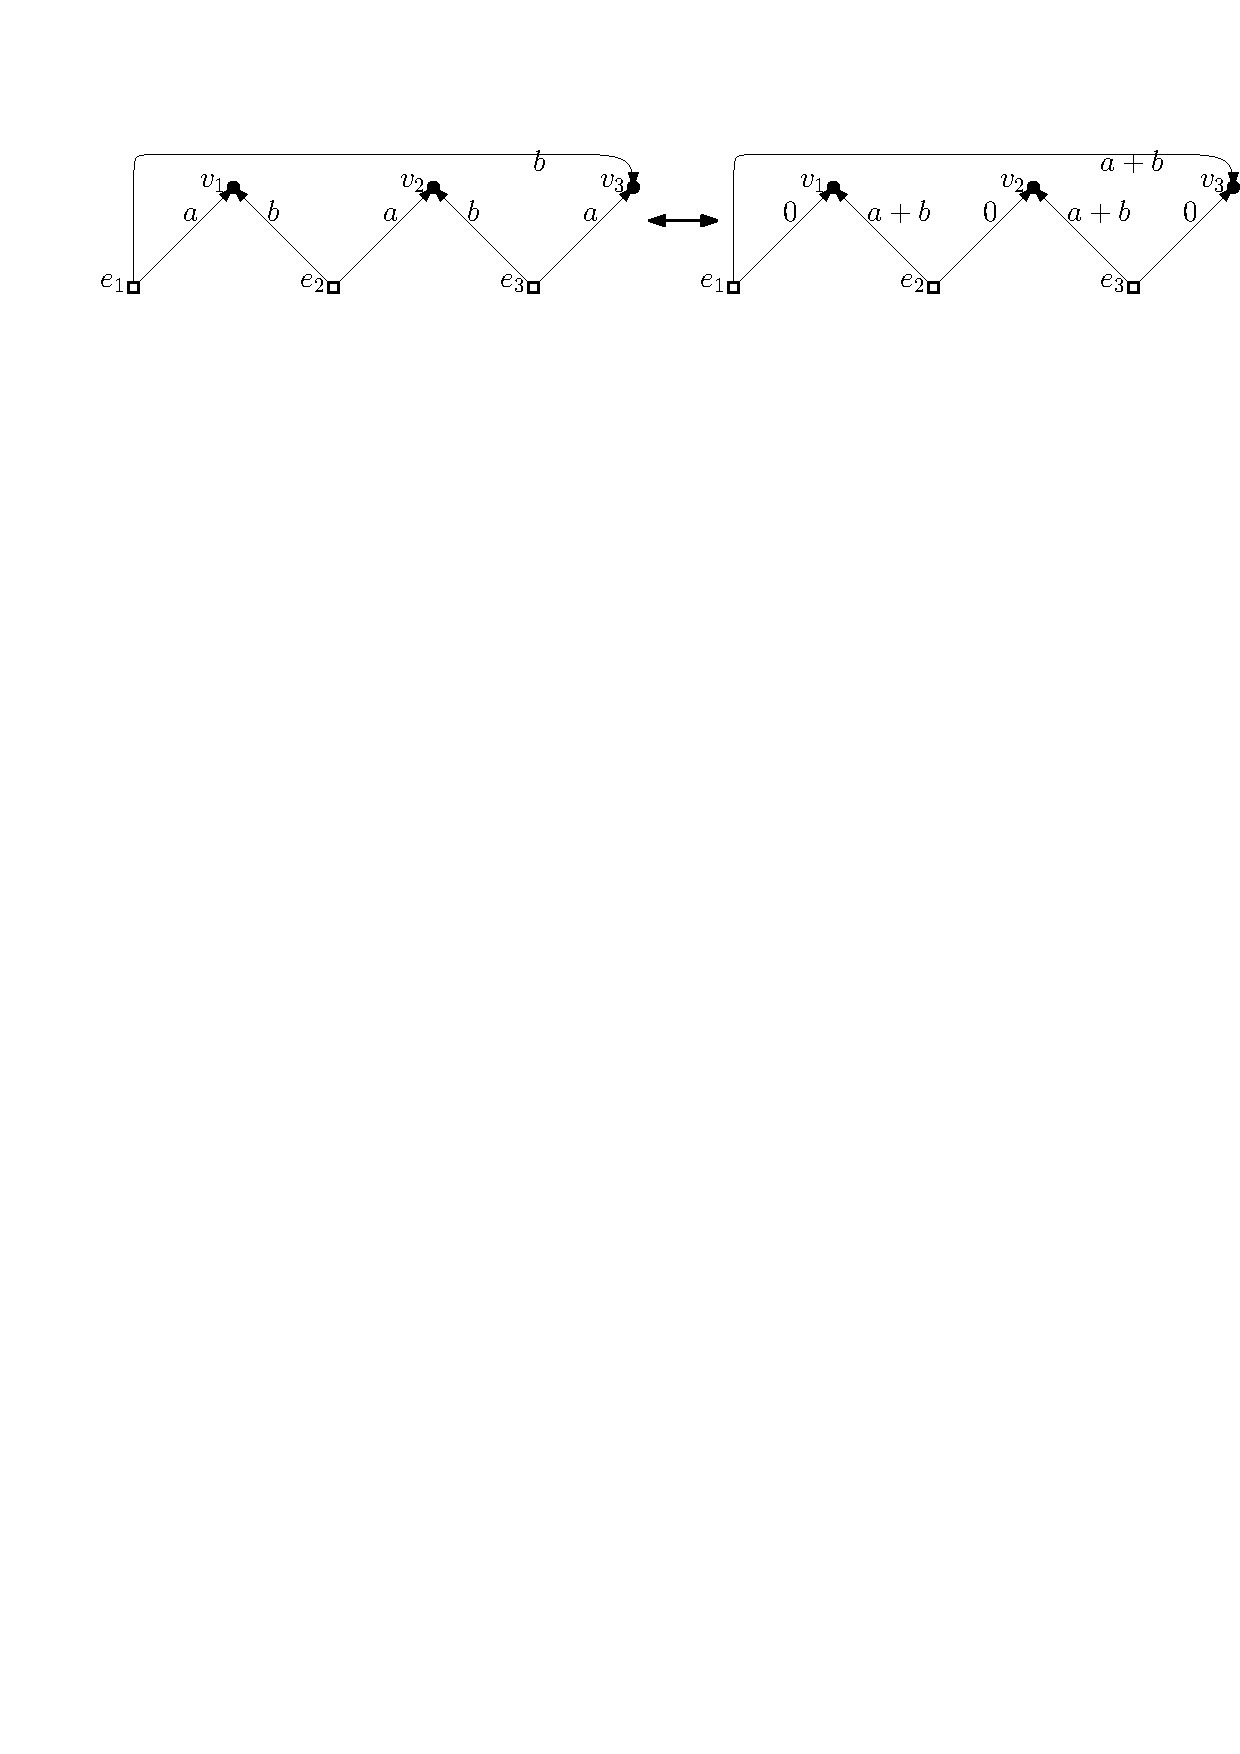
\includegraphics[width=1\textwidth]{K_kreis.pdf}
\caption{Wir können einen Schnyder-Zykel umkehren, wenn er nur aus V-Schritten besteht. Die Kapazitäten werden nicht überschritten und durch die Konten $v$ und $e$ fließt gleich viel Schnyder-Fluss. Merke, dass hier zwei Schnyder-Zykel mit Kapazitäten $a$ und $b$ abgebildet sind.}
\label{K_turn}
\end{figure}

\begin{definition}[Schnyder-Zykel und alternierende Zykel]
Sei $E_C = \{S_1\cup \ldots \cup S_n\}$, sodass alle $S_i$ V- oder F-Schritte sind und $S_i$ und $S_{i+1}$ zyklisch aufeinander folgen. Wir nennen $E_C$ einen \textit{Schnyder-Zykel} und seine Kapazität $|E_C|$ entspricht der minimalen Kapazität aller enthaltenen V- und F-Schritte. Wir nennen Schnyder-Zykel und die weiter unten definierten Zykel in Ecken- und Zuweisungs-Fluss \textit{alternierende Zykel} auf $\tilde{\varphi}$.
\end{definition}

Ein Schnyder-Zykel mit Kapazität 1 in $\mathcal{N}_G$ entspricht einem gerichteten Zykel einer $\alpha_s$-Orientierung. Insbesondere finden wir also zu essentiellen Zykeln bezüglich $\alpha_s$-Orientierungen auch Schnyder-Zykel mit Kapazität 1 in korrespondierenden Schnyder-Flüssen.

\begin{remark}
Wir können den fraktionalen Anteil des Schnyder-Fluss vollständig mit Schnyder-Zyklen der passenden Kapazitäten überdecken, ohne dabei neue fraktionale Teile zu erzeugen. Dies ist möglich, da wir den Fluss in Pfade aufteilen können. Da die Kanten, von der Quelle und zu Senke, gesättigt sind, reicht es die Pfadstücke zwischen den Kanten-Knoten und Gebiets-Knoten bzw. Knoten-Knoten zu betrachten. Aus diesen fraktionalen Pfadstücken können wir nun Schnyder-Zykel bilden. Dies wirft die folgenden Fragen auf, die wir allerdings hier nicht beantworten werden.

\begin{itemize}
\item Ist es möglich die Schnyder-Zykel so zu bilden, dass zu jedem ein korrespondierender essentieller Zykel auf $G+G^*$ existiert, wenn wir zulassen, dass auch ganzzahlige Pfade aufgeteilt werden?
\item Angenommen dies ist möglich, muss dann $\tilde{\varphi}_s$ eine Linearkombination aus ganzzahligen Schnyder-Flüssen sein?
\end{itemize}
\end{remark}

Die nächste Definition zeigt einen Weg auf, wie man mithilfe der alternierenden Zykel einen neuen zulässigen Fluss konstruieren kann.

\begin{definition}[Umkehrung eines Schynder-Zykels]
Sei $E_C = \{S_1\cup \ldots \cup S_n\}$ Schnyder-Zykel mit Kapazität $a=|E_C|$. Wir können einen Schritt $S_i$ umkehren, indem wir Fluss mit Kapazität $a$ vom ersten Teil der Kanten auf den zweiten Teil verschieben. Die \textit{Umkehrung} von $E_C$ erfolgt nun, indem wir jeden Schritt $S_i \subset E_C$ umkehren (vergleiche Abbildung \ref{K_turn}).
\end{definition}

Die Schnyder-Zykel, die nur aus V-Schritten bestehen, können wir umkehren, indem wir den Fluss in $\tilde{\varphi}_s$ wie in Abbildung \ref{K_turn} verändern. Die Kapazitäten der Kanten werden nicht überschritten und durch die Knoten-Knoten und Kanten-Knoten fließt gleich viel Schnyder-Fluss wie zuvor. Der resultierende Fluss ist somit weiterhin zulässig.

\begin{figure}[h]
\centering
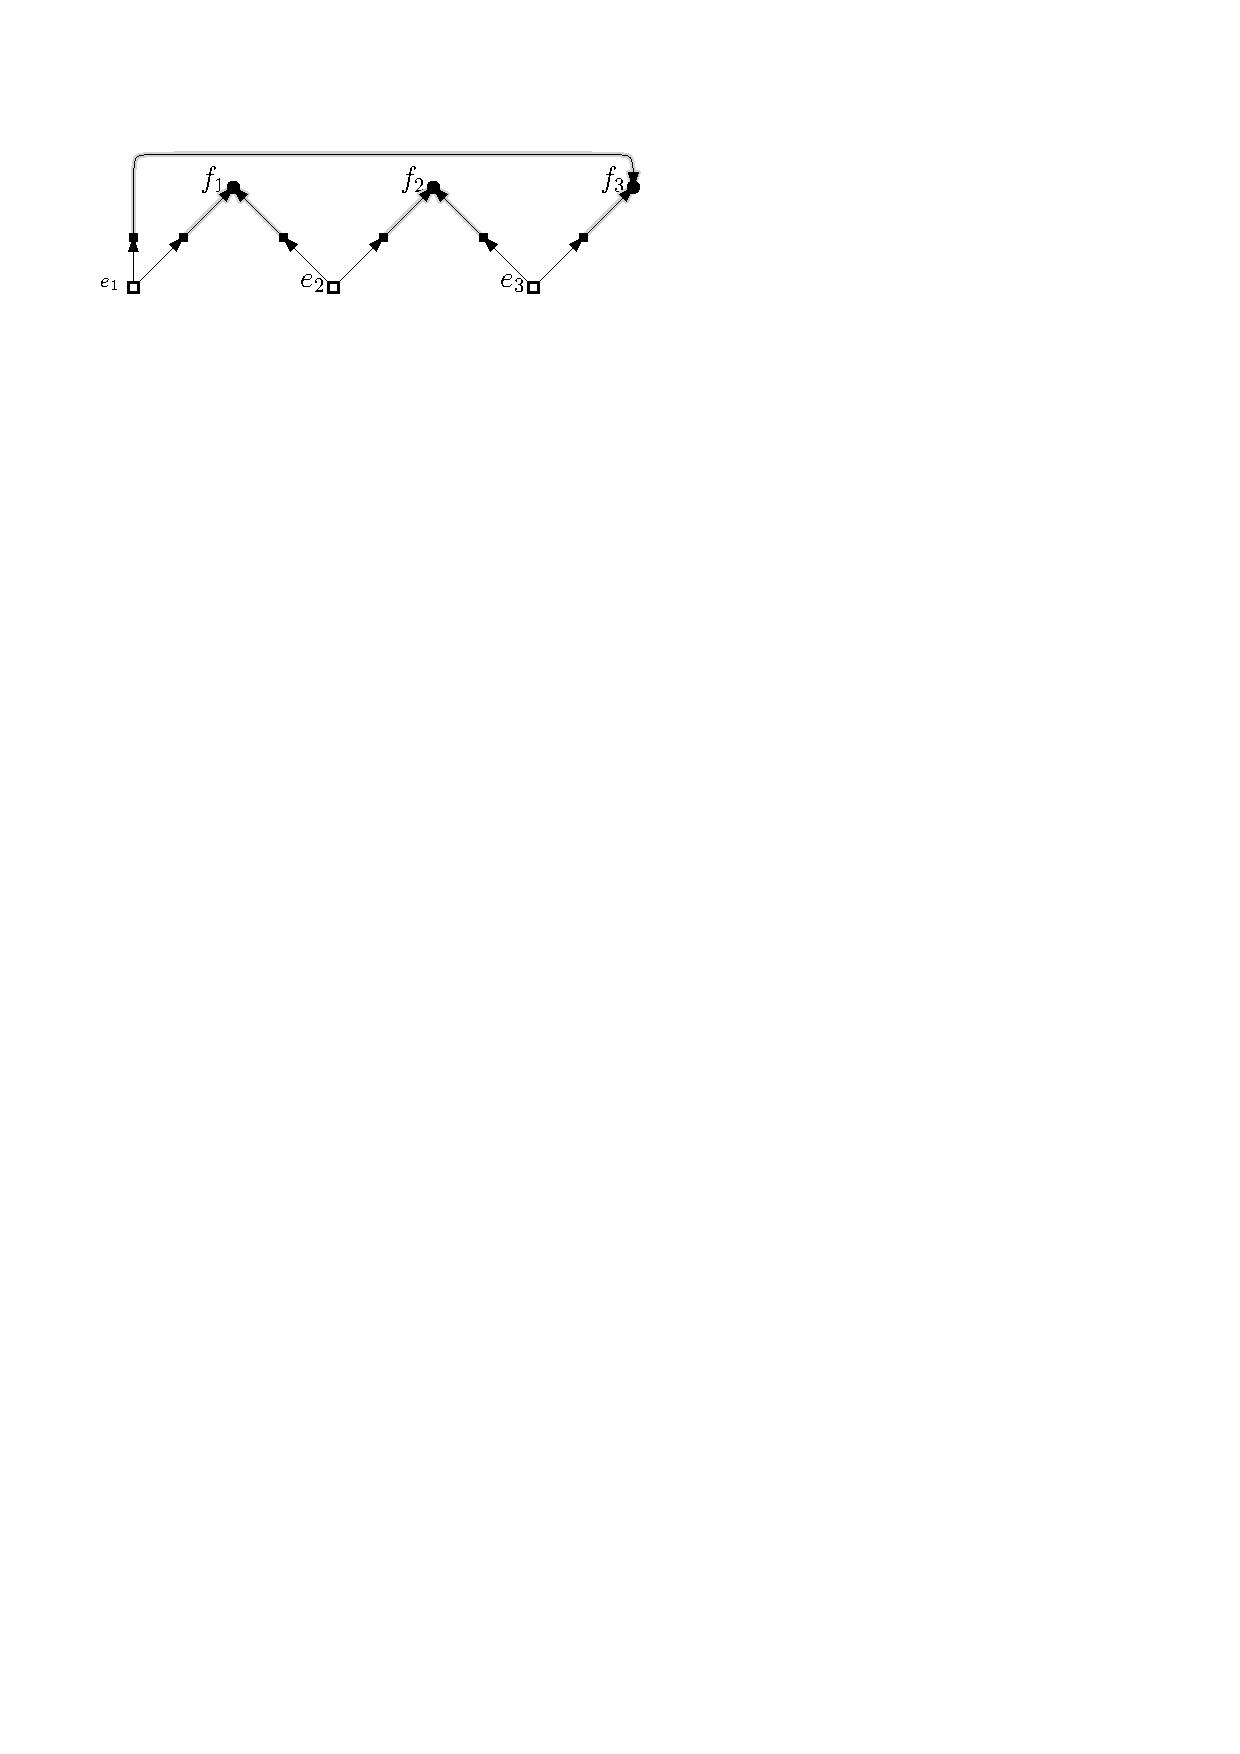
\includegraphics[width=0.7\textwidth]{G_kreis.pdf}
\caption{Wir können einen Schnyder-Zykel der F-Schritte enthält nicht umkehren, ohne auch den FAA-Fluss anzupassen, da wir sonst die Kapazitäten der Kanten überschreiten. Die grau unterlegten Kanten sind von $\tilde{\varphi}$ gesättigt.}
\label{G_turn}
\end{figure}

Betrachten wir einen Schnyder-Zykel, der nur aus F-Schritten besteht. So ein Fluss ist in Abbildung \ref{G_turn} dargestellt. Das Problem bei der Umkehrung ist, dass die Kanten zwischen den kleinen Quadraten und inneren Gebieten von einem zulässigen Fluss $\tilde{\varphi}$ gesättigt werden. Somit müssen wir, wenn wir den Zykel umkehren wollen, auch den FAA-Fluss $\tilde{\varphi}_F$ anpassen. Wir definieren analog zu oben alternierende Zykel auf dem Ecken- und Zuweisungsfluss. Beispiele sind in Abbildung \ref{combined_face_alt_cycle} zu sehen.

\begin{definition}[Z-Zykel und C-Zykel]
Wir nennen $E_C=\{S_Z \cup S'_Z\}$, mit  $S_Z = \{(s_2,w_1),(w_1,w_2),(w_2,v_1^*),(v_1^*,s_d)\}$ und $S'_Z=\{(s_2,w'_1),(w'_1,w'_2),(w'_2,v^{'*}_1),(v^{'*}_1,s_d)\}$ einen \textit{Z-Zykel} mit Kapazität $a$, falls gilt: 
$$\text{min}(\tilde{\varphi}_s(\{S_Z\}) = a > 0 \text{ und } \text{max}(\tilde{\varphi}_s(\{S'_Z\}) \leq 1 - a.$$
Wir nennen $E_C=\{C_Z \cup C'_Z\}$, mit  $C_Z = \{(s_2,w^1_1), (w^1_1,w^1_2), (w^1_2,w^1_3), (w^1_3,w^1_4), (w^1_4,w^2_3), $ $(w^2_3,w^2_4), \ldots (w^k_4,q),(q,f),(f,t_2)\}$ und analogem $C'_Z$ einen \textit{C-Zykel} mit Kapazität $a$, falls gilt: 
$$\text{min}(\tilde{\varphi}_s(\{C_Z\}) = a > 0 \text{ und } \text{max}(\tilde{\varphi}_s(\{C'_Z\}) \leq 1 - a.$$
\end{definition}

\begin{figure}[b!]
\centering
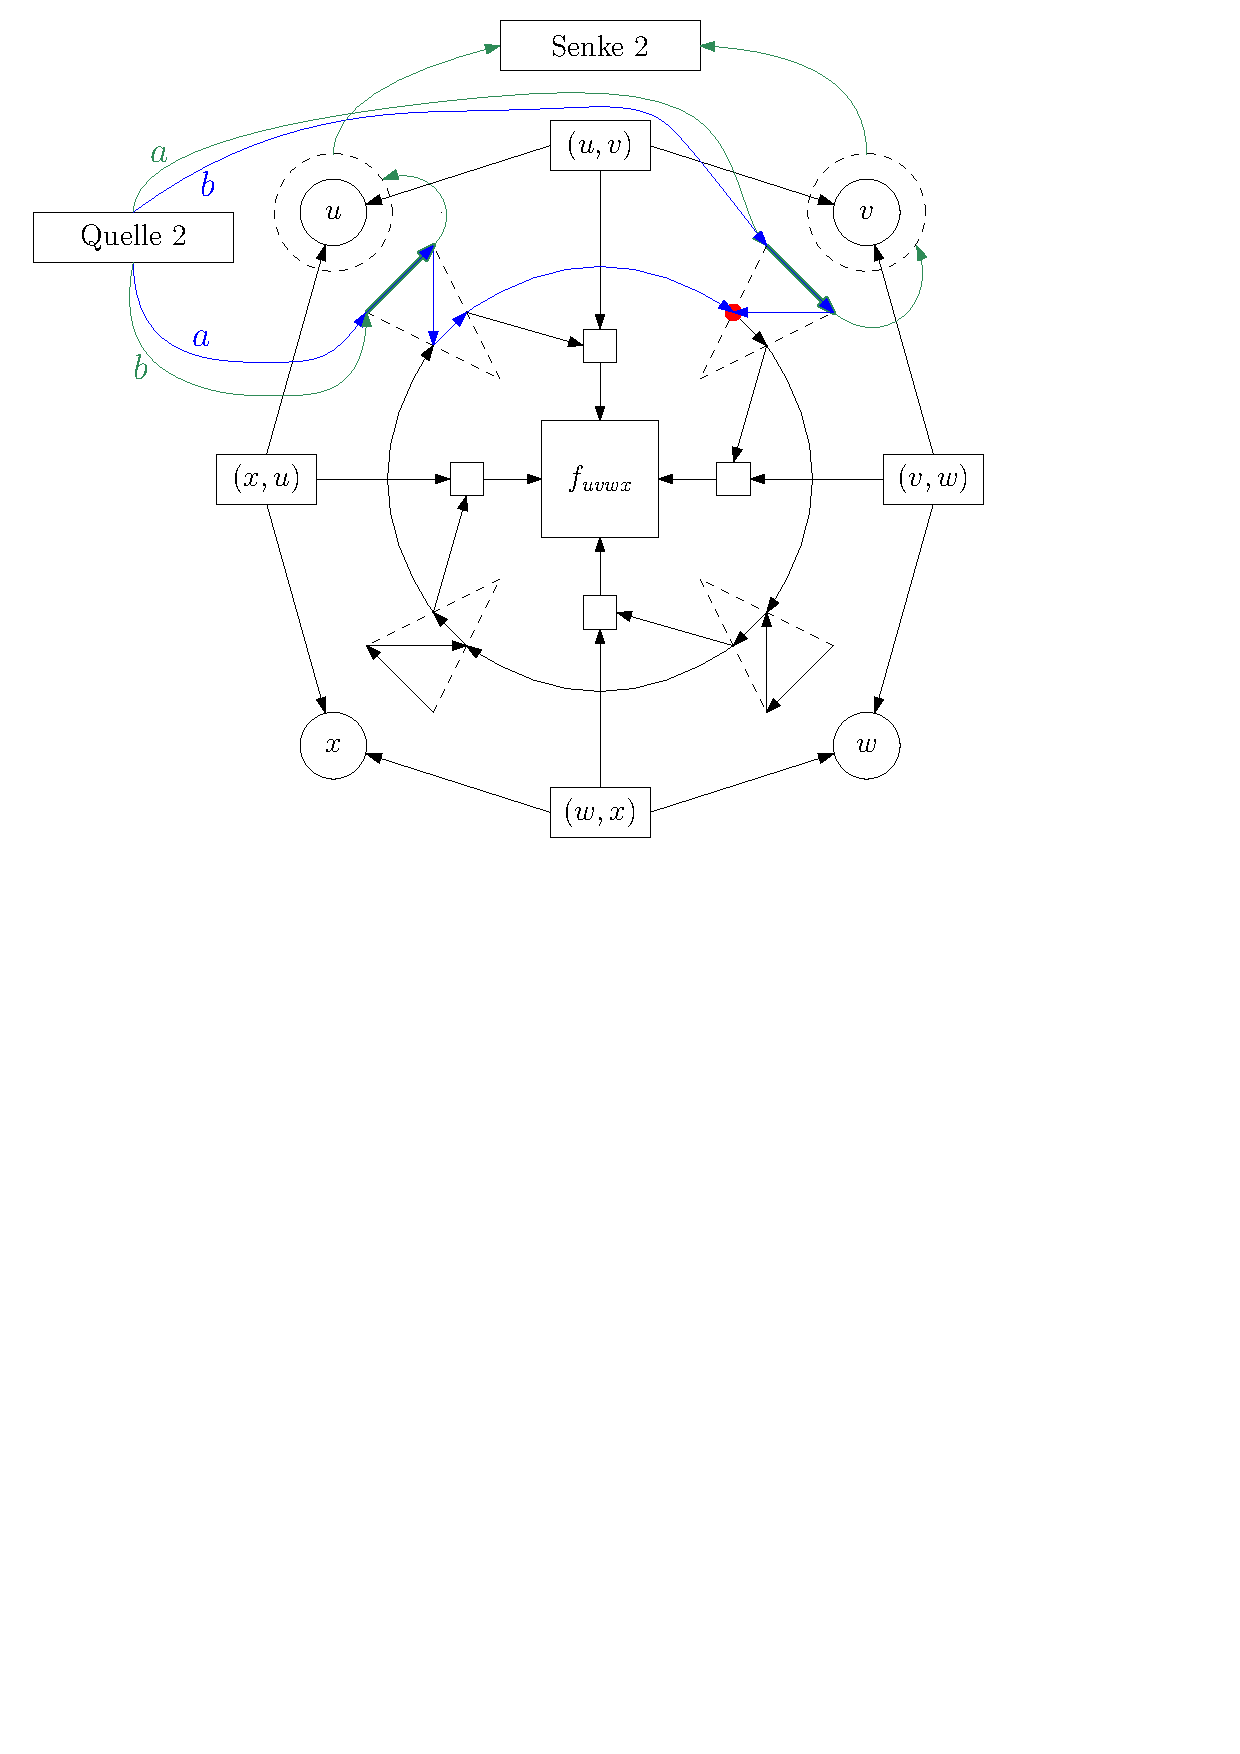
\includegraphics[width=0.8\textwidth]{combined_face_alt_cycle.pdf}
\caption{Ein Beispiel von zwei C-Zykeln (blau) und zwei Z-Zykeln(grün). Merke, dass es sich hier jeweils einmal um Zykel mit Kapazität $a$ und jeweils einmal um Zykel mit Kapazität $b$ handelt. Die C-Zykel führen in diesem Beispiel nur bis zu einem Winkeldreieck (roter Punkt). Falls $a+b=1$ gilt und durch einen der beiden, von den Z-Zykel genutzen Dummy-Knoten kein weiterer Zuweisungs-Pfad führt, können wir jeweils einen der beiden Zykel umkehren und erhalten einen ganzzahligen Fluss.}
\label{combined_face_alt_cycle}
\end{figure}

\begin{remark}
Die hier eingeführten Definitionen führen zu deutlich längeren gleichgerichteten Kantenfolgen als zuvor. Es können allerdings auch kürzere Formen von Z- und C-Zykel auftreten. Ein Z-Zykel kann schon in einem Dummy-Knoten enden. Ein C-Zykel kann entweder in einem inneren Gebiet oder am dritten Knoten $w_3$ eines Winkel\-dreiecks enden. In keinem der beiden Fälle müssen die Längen von erstem und zweitem Teil übereinstimmen.
\end{remark}

Analog zu oben ist es möglich, den fraktionalen Anteil von Ecken- und Zuweisungsfluss jeweils mit alternierenden Zykeln zu überdecken. In den Lösungen für $\mathcal{N}_G$, die mit dem in Kapitel \ref{the_program} vorgestellten Programm errechnet wurden, finden sich in allen drei Fluss-Typen solche Zykel. Durch schrittweises Umkehren war es uns auf kleineren Beispielen möglich, so ganzzahlige Lösungen zu konstruieren. Ein Ausschnitt aus einem Beispiel ist in Abbildung \ref{combined_face_alt_cycle} zu sehen.

\begin{figure}[b]
\centering
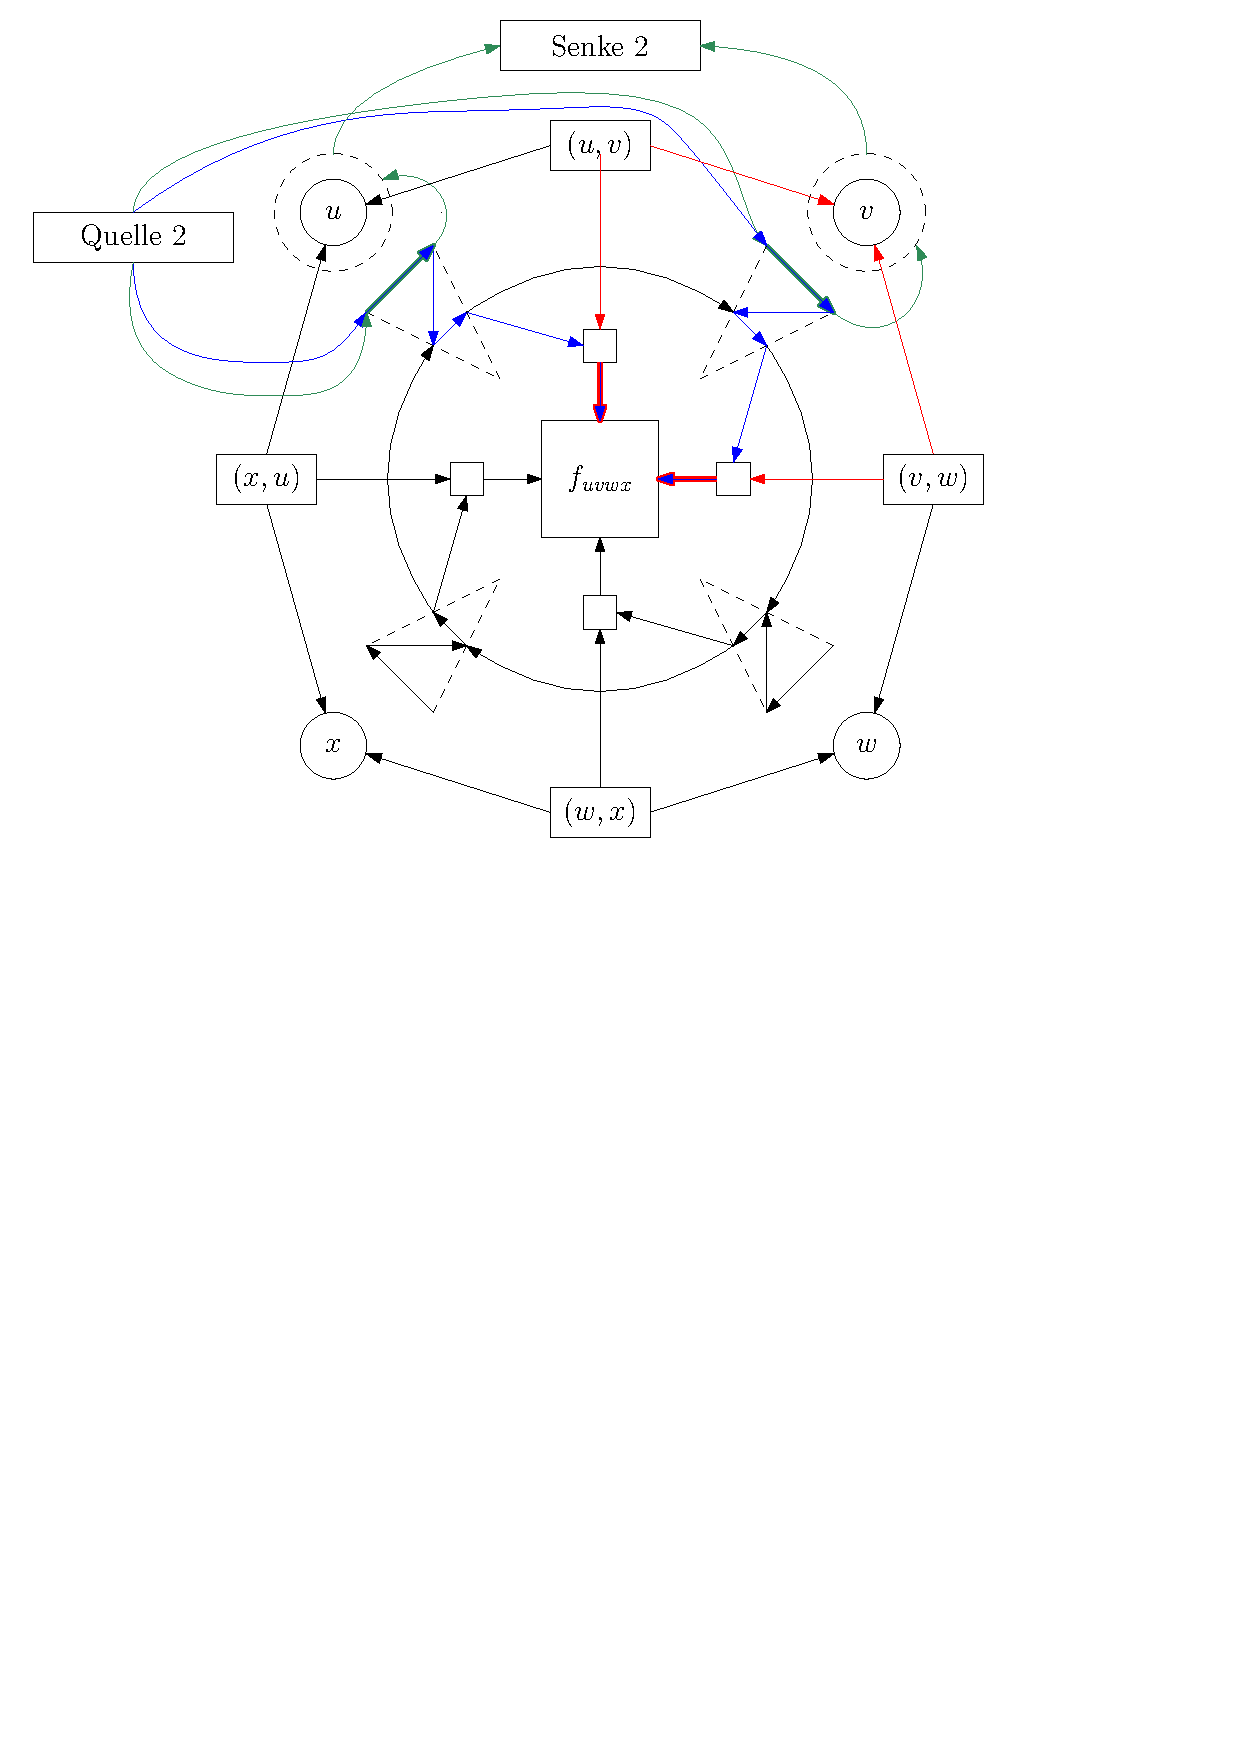
\includegraphics[width=0.8\textwidth]{combined_face_alt_cycle2.pdf}
\caption{Falls durch einen der Dummy-Knoten kein weiterer Zuweisungs-Pfad führt, können wir die Zykel so umkehren, dass wir einen ganzzahligen Fluss erhalten. Alle eingezeichneten Flüsse haben Stärke $1/2$. Die dicken Kanten sind somit ausgelastet.}
\label{combined_face_alt_cycle2}
\end{figure}


\begin{example}
Kommen wir zurück zu einen Schnyder-Zykel, den wir umkehren wollen. Betrachten wir den Fall, dass der Zykel nur durch einen Gebiets-Knoten führt. Wir müssen also einen oder mehrere Ecken-Zykel finden, die wir parallel zum Schnyder-Zykel umkehren können, sodass die Kapazitäten an den kleinen Quadraten nicht überschritten werden. In Abbildung \ref{combined_face_alt_cycle2} ist so eine Situation dargestellt. Nehmen wir an, dass auf allen eingefärbten Kanten ein Fluss mit Stärke 1/2 fließt. Wie man hier sieht, müssen wir nun aber zusätzlich noch mindestens auf die äußeren Winkelkanten achten, an denen sich Zuweisungs- und Ecken-Zykel überschneiden. Wie in Proposition \ref{claim_non_int} festgehalten, sind diese Fälle die relevanten. Wenn nur zwei Flusstypen nicht-ganzzahlig sind, können wir eine ganzzahligen Lösung konstruieren. Für die alternierenden Zykel in der Abbildung ist die gleichzeitige Umkehrung möglich, falls durch einen der beiden Dummy-Knoten kein weiterer Pfad läuft.
\end{example}

In einer nicht-ganzzahligen Lösung auf einem Netzwerk, dass eine ganzzahlige Lösung zulässt, müsste es einen Weg geben, über das Umkehren von alternierenden Zykeln zu einer ganzzahligen Lösung zu kommen. Nehmen wir jedoch an, dass es keine ganzzahlige Lösung gibt, dann könnten wir auf diesem Weg zu einem Widerspruch gelangen und somit Vermutung \ref{int_conj} beweisen. Wir haben dies für einige Sonderfälle zeigen können, doch noch keinen allgemeinen Beweis gefunden. Wir formulieren darum eine weitere Frage:
\begin{itemize}
\item Falls wir einen (essentiellen) Schnyder-Zykel $E_C$ gegeben haben, existiert dann eine Menge aus C- und Z-Zykeln (und potentiell weiteren Schnyder-Zyklen), sodass die gemeinsame Umkehrung dieser Zykel dazu führt, dass der fraktionale Flussanteil kleiner wird?
\end{itemize}
Weil wir mit unseren Mitteln diese Frage nicht beantworten konnten, beenden wir an diesem Punkt die Erläuterung der Beweisansätze und müssen Vermutung \ref{int_conj} und Vermutung \ref{faa_conj} unbewiesen lassen.
